% ============================================================
% Comment on Ma, Geng & Zhong (2026), Forests
%
% In-place edits 2026-10-07 (editor major revision):
%   A. Title softened: "Not Robustly Identified" replaces "No Effect".
%   B. Pencil-test claim fixed: removed factually wrong claim that a
%      straight line fits all post-period CIs; replaced with correct
%      argument about pre-period trend ambiguity.
%   C. Abstract, Discussion, Conclusion softened throughout.
%   D. Extreme hot-days aggregate ATT added to Results text; Figure 3
%      updated from 2x2 to 3+2 layout adding extreme hot-days panel.
%   E. Missing-obs treatment documented; buffer corrected 20km -> 50km.
%   F. Data and code availability statement added.
%   G. Description of Ma et al.'s estimator corrected.
% Previous version saved in _old/ as comment_nfcp_v6.tex.
%
% Updated from comment_nfcp_v5 to comment_nfcp_v6 on 2026-07-25.
% Main changes in this version:
%   - All results updated from final Stata pipeline run (2026-07-25).
%     Stata did_imputation used for BJS without controls (correct BJS
%     variance); Stata csdid used for CS and CS-DR; Python BJS with
%     controls unchanged.
%   - Year range corrected: 2000-2025 (7,150 city-years).  Year 1999
%     was synthetic test data; dropped from all analysis.
%   - BJS stage-1 now uses all clean observations (never-treated + pre-
%     treatment periods of eventually-treated), following the standard
%     BJS (2024) definition.  Appendix A2 (all-clean vs. never-treated
%     comparison) dropped as moot; former A3 (station vegetation)
%     renumbered A2.
%   - New finding: BJS without controls shows significant positive LST
%     effect (+0.262 C, p<0.01), consistent with selection into NFCP
%     by cities on warmer trajectories.  Covariate adjustment absorbs
%     this; BJS with controls is null.
%   - CLCD forest: BJS without controls at 20km is now significant
%     negative (-0.425 pp, p<0.01); CS and CS-DR are null.
%   - Axis labels and panel titles added to all figures in LaTeX.
%   - Figures 2 and 3 now use Stata-generated PNGs.
% Previous version saved in _old/ as comment_nfcp_v5.tex.
%
% In-place edits 2026-07-31 (instructions_11.txt):
%   - Dropped BJS without controls from Table 1 and Figure 2 entirely.
%     Note in text and table caption that BJS without controls fails
%     parallel pre-trends and is not presented.
%   - Figure 2 (fig:bjs_nocontrols) deleted.
%   - Figure 4 restructured: dropped LST station panels (left column);
%     inserted NDVI and tree cover station panels (from old Appendix A2).
%   - Appendix A2 (fig:stationveg) deleted; content merged into Figure 4.
%   - Station analysis text updated to match new Figure 4 layout.
%   - Results, Discussion, Conclusion revised: removed selection narrative;
%     added note on BJS pre-trend failure motivating covariate adjustment.
%   - Style revision: active voice, present tense, brevity throughout.
%   - Code changes (code changes require user re-run):
%     run_analysis_v6.py, run_analysis_stata_v1.py,
%     run_station_analysis_stata_v1.py: added light gray vertical line at t=0.
%     run_station_analysis_stata_v1.py: restricted ATT to t=0..10 window.
%     run_one_spec_station.do: changed allhorizons to horizon(0 10) for BJS.
%
% Minor updates 2026-07-27 (in-place, no version bump):
%   - All figures regenerated from 2026-07-27 pipeline run with updated
%     style: s1mono scheme, CI whiskers (not shading), dots only (no
%     connecting lines), labels embedded in figure panels.
%   - All numerical results confirmed unchanged vs. 2026-07-25 run.
%   - Fig 4 tabular: added singlespace wrapper and @{}cc@{} column spec
%     for consistency with Figs 1-3.
%   - Appendix A2 caption: added "Dots are point estimates" for
%     consistency.
%
% (Older history below for reference)
% Updated comment_nfcp_v5 on 2026-07-19:
%   - Data section: corrected year range and city-universe paragraph.
%   - Methods: clarified BJS stage-1 and SE footnote.
%   - Appendix A3 added: station vegetation.
% Updated from comment_nfcp_v4 to comment_nfcp_v5 on 2026-07-18.
% Updated from comment_nfcp_v3 to comment_nfcp_v4 on 2026-07-18.
%
% NOTE: Replace \documentclass{article} with the MDPI Forests template
% class (mdpi.cls) before submission.
% ============================================================

\documentclass[12pt]{article}
\usepackage[utf8]{inputenc}
\usepackage[T1]{fontenc}
\usepackage[margin=1in]{geometry}
\usepackage{setspace}
\doublespacing
\usepackage{natbib}
\bibpunct{(}{)}{;}{a}{,}{,}
\usepackage{booktabs}
\usepackage{amsmath}
\usepackage{graphicx}
\usepackage{subcaption}
\usepackage{hyperref}
\usepackage{caption}
\usepackage{placeins}
\usepackage{gensymb}
\newcommand{\noclaude}[1]{#1}
\newcommand{\forclaude}[1]{}
\newcommand{\foruser}[1]{}

\graphicspath{{../analysis/figures/}}

\title{The Effect of China's National Forest City Program on Urban Heat
       Is Not Robustly Identified: Comment on \citet{Ma2026} and Demonstration of the Use of Coding Agents for Replication Studies}

\author{Matthew Turner\footnote{Brown University, Department of Economics, Box B, Brown University, Providence, \textsc{ri} 02912. email: \texttt{Matthew\_Turner@Brown.edu}. Also affiliated with PERC, IGC, NBER, PSTC.}}

\date{October 2026}

\begin{document}

\maketitle

\begin{singlespace}
\begin{abstract}
Using a staggered adoption difference-in-differences design,
\cite{Ma2026} claim that China's National Forest City Program (NFCP) reduces extreme heat days by about three per year in designated cities. However, their data appear to violate parallel trends, they rely on an estimator known to be biased, they provide no evidence for the increase in forest cover that would cause cooling, and their main specification includes plausibly endogenous controls. In the absence of a public replication package, we rely on coding agents to conduct an otherwise impractical replication exercise. Using slightly different data than the original, we replicate their research design using three heterogeneity robust estimators. Point estimates indicate that the NFCP increased extreme heat days and we reject that it decreased them. We also estimate slightly positive effects on mean summer temperature, although these estimates are imprecise and their 95\%CI contains zero. We conclude that the \citeauthor{Ma2026}results are not robustly identified and that they probably reflect unobserved features or trends in cities that select into the program.
\end{abstract}
\end{singlespace}

\textbf{Keywords:} National Forest City Program; urban heat island;
difference-in-differences; staggered adoption; MODIS; land surface
temperature; NDVI; forest cover

% ------------------------------------------------------------------
\section{Introduction}
\label{sec:intro}
% ------------------------------------------------------------------

\citet{Ma2026} use a staggered adoption difference-in-differences design on city-year panel of 243 Chinese prefecture-level cities during 2000--2023 to argue that designation under China's National Forest City Program (NFCP) reduces the annual count of extreme heat days ($\geq 35^\circ$C) by approximately three per year in designated cities.

There are four reasons to regard this conclusion with skepticism.  First, \citeauthor{Ma2026} give no evidence that the NFCP increased urban green cover. Second, their main event-study plot shows a decreasing pre-trend, suggesting a violation of the parallel trends assumption on which difference in differences estimation relies. Third, their main estimates use a TWFE regression known to be biased under heterogeneous treatment effects \citep{GoodmanBacon2021}. Fourth, their main regression conditions on a long list of covariates, per capita GDP among them. Because per capita GDP is plausibly correlated with the propensity to apply for NFCP designation and temperature trends (e.g. from industrial or commercial development) treatment effect estimates may be confounded.

We repeat the \citet{Ma2026} evaluation of the NFCP using three heterogeneity robust estimators.  First, the \citeauthor{Borusyak2024} (BJS) imputation estimator with covariate adjustment \citep{Borusyak2024}. Second, the
Callaway--Sant'Anna estimator (CS) \citep{CS2021}, which does not permit covariate adjustment. Third, its doubly robust variant (DR) \citep{SantAnnaZhao2020}, with covariate adjustment.\footnote{BJS without covariate adjustment does not satisfy the parallel pre-trends condition and we do not report it.}

We find no evidence that the NFCP increased forest cover. If anything, satellite-measured vegetation near city centers declines after NFCP designation. We also find that, using a satellite based temperature measure, our point estimates for the effect of the NFCP on summer mean temperature are slightly positive, indistinguishable from zero, and precise enough to allow us to reject a decrease in summer mean temperature of more than about 0.2\degree C.    Repeating these estimations at the weather station-year level (rather than city-year), and using the sample of 99 cities for which weather station data is publicly available, we find an about 0.1\degree C increase in mean summer temperature. If we use the same extreme same heat days outcome as \citet{Ma2026}, instead of satellite or instrument based measures of summer temperature, we find that NFCP increased annual hot days by about 1.6.

% ------------------------------------------------------------------
\section{Comment on Identification Strategy}
\label{sec:id}
% ------------------------------------------------------------------

\citet{Ma2026} implement a staggered adoption differences in differences design. Their main estimates use OLS-TWFE with a treated $\times$ post indicator.  With heterogenous treatment effects, this estimator may be biased \citet{GoodmanBacon2021}. The literature proposes a number of heterogeneity robust estimators for staggered adoption designs.  We implement three of them below, and find that their result disappears or is reversed.

The main regression in \citet{Ma2026} conditions on a set of time-varying city-level controls, including per capita GDP.  Per
capita GDP is plausibly correlated with both the propensity to apply for NFCP
designation and with temperature trends independent of the program. Therefore, the effects of this control may be confounded with the effects of the treatment.

In a difference-in-differences design, the identifying assumption is parallel
trends: absent designation, treated and control cities would have followed the same outcome path.  Researchers include covariates to restore conditional parallel trends when the unconditional version fails (or to improve precision when it holds). We find that BJS without covariate adjustment shows pre-designation LST coefficients that diverge from zero, indicating that NFCP and control cities are on different pre-designation temperature trajectories.
Conditioning on pre-determined city characteristics (latitude, longitude, and
log pre-treatment population) absorbs this imbalance.

% ------------------------------------------------------------------
\section{Data and Methods}
\label{sec:data}
% ------------------------------------------------------------------

\subsection*{Data}

We draw our city-level panel from the
United Nations World Urbanization Prospects (WUP 2018) dataset \citep{UN2018}. These data describe cities with populations of at least 300,000 and WUP centroids anchor all satellite data extractions.  Treatment is a binary indicator equal to one for city $i$ in all years at or after its first NFCP designation, constructed from annual lists published by the National Forestry and Grassland Administration.  The panel covers 275 prefecture-level cities observed from 2000 to 2025 (7,150 city-years); 149 hold NFCP designation across 17 cohorts (2004--2022) and 126 remain never-treated. We extract all outcomes at buffer radii of 5, 10, and 20~km from the city centroid.  Main estimates use the 20~km buffer; 5~km results are reported in Table~\ref{tab:att} and in Appendix A1.

China has approximately 337 prefecture-level administrative units.  Our sample
of 275 is smaller for two reasons.  First, the WUP includes only agglomerations
exceeding its 300,000-resident threshold; smaller prefecture-level units fall
below it.  Second, we exclude county-level cities that appear in the WUP because the NFCP programme targets prefecture-level units
exclusively.

To measure temperature, we use MODIS 8-day composite LST
at 1~km resolution \citep{Wan2021} (downloaded, NASA EOSDIS, June 2026.).  For each city-year we average June--August pixels within each buffer around the city center, excluding fill values. Note two deviations from \citet{Ma2026}. First, the \citet{Ma2026} outcome is calculated on the basis of prefecture boundaries rather than disks centered on the city center. Second, the  \citet{Ma2026} outcome is a weather station derived measure of  days per year warmer than 35\degree C rather than a sattelite based summer average tenperature. We will verify our conclusions are robust the calculating outcomes using prefecture boundaries and a subsample of weather station data to match \citet{Ma2026} more closely.  We cannot exactly match the \citet{Ma2026} sample becasue the full sample of weather stations is not publicly available.

We consider three satellite based measures of urban vegetation and tree cover. First, MODIS reports the Normalized Difference Vegetation Index (NDVI) monthly  composites at 1~km
resolution \citep{Didan2021}(downloaded, NASA EOSDIS, June 2026).  From these data we compute mean July NDVI for each city-year. Second, the MODIS Vegetation Continuous Fields product reports annual tree canopy cover at 250~m resolution \citep{DiMiceli2021} (downloaded, NASA EOSDIS, June 2026).  From these data we compute mean canopy fraction for each city-year. Finally, the CLCD reports annual Landsat-based land cover classifications at 30~m resolution \citep{Yang2021} (Zenodo record 18180184, 1985--2025, downloaded June 2026). From these data we compute the forest pixel share for each city-year.  With a 30~m resolution, the CLCD detects land cover changes not visible in the lower resolution MODIS data.

The panel is largely complete.  Among the 7,150 city-years, MODIS LST at 5~km
has 286 missing observations (4.0\%), concentrated in persistently cloudy
cities; LST at 20~km, NDVI, and tree cover have fewer than 30 missing
observations combined.  CLCD is complete for all 7,150 city-years.

We supplement our satellite based city-year analysis with a second city-year analysis in which outcomes are derived from weather station records and their nearest satellite pixels rather than averaged over buffer zones.  We use GHCN-Daily records \citep{Menne2012}, the same data source as \citet{Ma2026}.  We retain stations within 50~km of a city centroid with at least 30 valid daily maximum temperature readings per year; city-years for which no station meets this threshold are excluded from the estimation sample.  Where a city has multiple qualifying stations, all outcomes are averaged across stations to yield one observation per city-year.  The station sample covers 52 treated cities (16 cohorts) and 47 never-treated cities.  Temperature outcomes are summer mean daily maximum temperature (Tmax, June--August) and the count of days with Tmax $\geq 35^\circ$C.  Vegetation outcomes are MODIS NDVI and tree cover extracted from the pixel closest to each station, and CLCD forest cover as the forest pixel share within a 100~m radius buffer around each station; where multiple stations exist within a city, these per-station values are averaged to one city-year observation.

\subsection*{Methods}

The \textit{BJS imputation
estimator} \citep{Borusyak2024} fits TWFE on untreated observations (never- and not-yet-treated units), imputes
counterfactual outcomes for treated units, and identifies treatment effects as observed minus imputed.  BJS without covariate adjustment fails the parallel pre-trends condition and we do not report it. \textit{BJS with controls} augments the first stage TWFE with covariate~$\times$~time
interactions for city latitude, longitude, and log pre-treatment population,
allowing cities in different settings or of different sizes to follow different time trends.  These covariates are pre-determined and time-invariant.  Because they are time-invariant,
entering them in levels would be collinear with city fixed effects; we
therefore interact each with five-year period-bin dummies.
The \textit{Callaway--Sant'Anna estimator} \citep[CS;][]{CS2021} compares each treatment cohort to never-treated cities at each event-time horizon without covariate adjustment.  Finally, the \textit{doubly robust estimator} \citep[DR;][]{SantAnnaZhao2020} is a variant of CS that allows for covariates.  DR conditions on the same pre-determined variables (latitude, longitude, and log pre-treatment population).  For each estimator we aggregate to an average post-period ATT as the simple mean of event-study coefficients at $t = 0, 1, \ldots, 10$,
with the mean of period-level clustered standard errors as a conservative SE
approximation.

The period-level standard errors for BJS with controls specifications (columns~1--2 of table \ref{tab:att}) are obtained from a stage-3 OLS of $\hat{\tau}_{it}$ on event-time dummies with standard errors clustered at the city level.  This treats the imputed counterfactuals as
known rather than estimated, and therefore does not implement the efficient
influence-function variance derived in \citet{Borusyak2024} (Section~4 of
the published version).  Because all BJS-with-controls temperature estimates
are far from any conventional significance threshold ($|z| \leq 0.3$), this
limitation does not affect any substantive conclusion.  Standard errors for DR (column~3 of table \ref{tab:att}) and CS (column~4 of table \ref{tab:att}) are from Stata's \texttt{csdid}, which implements the influence-function variance of \citet{SantAnnaZhao2020} and \citet{CS2021} respectively.

The code that organized the data and performed the estimations in this comment was written by a Claude agent. To validate the data processing pipeline, we first confirmed that all outcome values lay in plausible ranges. Second, for each raw data layer, we constructed a synthetic layer for which the final city-year level outcomes were known and verified that these values obtained. To validate the estimation routines, we first conducted all estimations twice, once using python estimation libraries, and once using stata estimation routines. We next gave a separate Claude agent, with no knowledge of the project, the final data set and a draft of this comment, and confirmed that the agent could reproduce results from these sources alone.


% ------------------------------------------------------------------
\section{Results}
\label{sec:results}
% ------------------------------------------------------------------

Table~\ref{tab:att} reports average post-period ATTs.  The \citet{Ma2026}
temperature result does not appear. BJS with controls gives $+0.032^\circ$C (95\%~CI $[-0.18,\;+0.24]$) at 20~km and $+0.016^\circ$C (95\%~CI $[-0.22,\;+0.25]$) at 5~km, both indistinguishable from zero.
DR gives $+0.016^\circ$C (95\%~CI $[-0.17,\;+0.21]$) and CS gives $+0.067^\circ$C (95\%~CI $[-0.12,\;+0.25]$). For reference, the mean absolute year-to-year change in summer mean LST across cities is $1.0^\circ$C; for hot days ($\geq 35^\circ$C) across stations it is $6.2$~days. In sum, no estimate of NFCP on temperature is statistically distinguishable from zero, point estimates are positive rather than negative, and magnitudes are small relative to normal annual variation.

The remaining two columns consider variants of our specification that more nearly resemble \citet{Ma2026}. Column 5 replicates the results of column 4 using an outcomes calculated on the basis of prefecture boundaries rather than 5 or 20km disks.  gives $+0.055^\circ$C (95\%~CI $[-0.12,\;+0.23]$), consistent with other results.

Column 6 replicates results in column 1 for the 99 cities with qualifying weather station data.  The analysis remains at the city-year level; where multiple stations fall within the 50~km buffer, outcomes are averaged across stations before estimation.  Temperature outcomes use station-measured Tmax and hot days rather than MODIS LST; vegetation outcomes use the nearest satellite pixel to each station rather than averaging over circular buffer zones.  Row 1 reports station summer mean Tmax and row 5 reports hot days ($\geq 35^\circ$C), the same outcome as \citet{Ma2026}.  As for all other columns, point estimates are small and indistinguishable from zero.



\begin{table}[t!]
\centering
\caption{Average post-period treatment effects ($t = 0$ to $t = 10$).
Each cell is the simple mean of event-study coefficients at
$t = 0, 1, \ldots, 10$.  Standard errors in parentheses are the mean of
period-level clustered standard errors.  95\% confidence intervals [ATT $\pm$ 1.96$\times$SE] are
shown in square brackets for LST and hot days.
Columns: (1)~BJS with controls at 20~km; (2)~BJS with controls at 5~km; (3)~DR with controls at 20~km; (4)~CS at 20~km; (5)~CS at prefecture-level geography; (6)~BJS with controls, outcomes from weather station records (city-year, averaged across stations).}
\label{tab:att}
\resizebox{\textwidth}{!}{%
\begin{tabular}{lcccccc}
\hline \hline
 & (1) BJS & (2) BJS & (3) DR & (4) CS & (5) CS & (6) BJS \\
 & w/ctrl, 20~km & w/ctrl, 5~km & 20~km & 20~km & pref & w/ctrl, stn \\
\midrule
LST ($^\circ$C)$^{\S}$ & $+0.032$ & $+0.016$ & $+0.016$ & $+0.067$ & $+0.055$ & $+0.114$ \\
               & $(0.106)$ & $(0.121)$ & $(0.097)$ & $(0.095)$ & $(0.087)$ & $(0.184)$ \\
               & $[-0.18,\;+0.24]$ & $[-0.22,\;+0.25]$ & $[-0.17,\;+0.21]$ & $[-0.12,\;+0.25]$ & $[-0.12,\;+0.23]$ & $[-0.25,\;+0.47]$ \\[4pt]
NDVI (index)  & $+0.002$ & $-0.001$ & $-0.000$ & $+0.000$ & $-0.001$ & $-0.019$ \\
               & $(0.002)$ & $(0.003)$ & $(0.002)$ & $(0.002)$ & $(0.002)$ & $(0.018)$ \\[4pt]
Tree cover (\%) & $+0.095$ & $+0.047$ & $-0.103$ & $-0.165$ & $-0.146$ & $-1.060$ \\
               & $(0.287)$ & $(0.380)$ & $(0.256)$ & $(0.263)$ & $(0.253)$ & $(0.998)$ \\[4pt]
CLCD forest (pp) & $-0.194$ & $-0.585^{*}$ & $-0.089$ & $-0.291$ & $-0.188$ & $-2.41$ \\
               & $(0.301)$ & $(0.319)$ & $(0.219)$ & $(0.212)$ & $(0.178)$ & $(2.07)$ \\[4pt]
Hot days (count) & --- & --- & --- & --- & --- & $+1.602$ \\
               & & & & & & $(2.062)$ \\
               & & & & & & $[-2.44,\;+5.64]$ \\[4pt]
\midrule
Covariates     & Y & Y & Y & N & N & Y \\
\hline \hline
\end{tabular}}

\flushleft
{\footnotesize
* $p < 0.10$, ** $p < 0.05$, *** $p < 0.01$.  Standard errors clustered at
the city level.  $\S$~In column~(6), the temperature row reports station-measured summer mean
daily maximum temperature (Tmax, $^\circ$C), not MODIS LST.}
\end{table}


Rows 2, 3, and 4 of table \ref{tab:att} report treatment effects of NFCP designation on measures of forest cover. Except for the outcome variables, all estimates are identical to those predicting temperature outcomes.
MODIS NDVI, tree cover, and CLCD forest cover show no post-designation
increase at any buffer radius.  In fact, CLCD forest share declines near city centers. BJS with controls at 5~km gives $-0.585$ pp ($SE = 0.319$, $p < 0.10$); CS and DR estimates are statistically null but uniformly negative.
These results indicate not merely that the NFCP fails to increase forest
cover, but that cities entering the program experience vegetation losses near
their centers.


Figure~\ref{fig:main} illustrates these findings.  The four panels show
BJS with controls event studies using outcomes averaged over 20~km radius disks centered on the city center.  The top-left panel (summer LST) shows point estimates that scatter around zero from the start of the pre-period through $t = 10$, with confidence intervals that contain zero throughout.  The remaining three panels show no obvious post-designation change in MODIS NDVI, MODIS tree cover fraction, or Landsat-derived CLCD forest cover. All of the outcomes are noisy and not obviously affected by NFCP designation. A possible exception is the CLCD based forest cover plot in the bottom right. Here, pre-trends look parallel and there is a weak decline in tree cover post treatment. In sum, these plots demonstrate that the findings in \cite{Ma2026} are not robust.

\begin{figure}[t!]
\centering
\begin{singlespace}
\begin{tabular}{@{}cc@{}}
  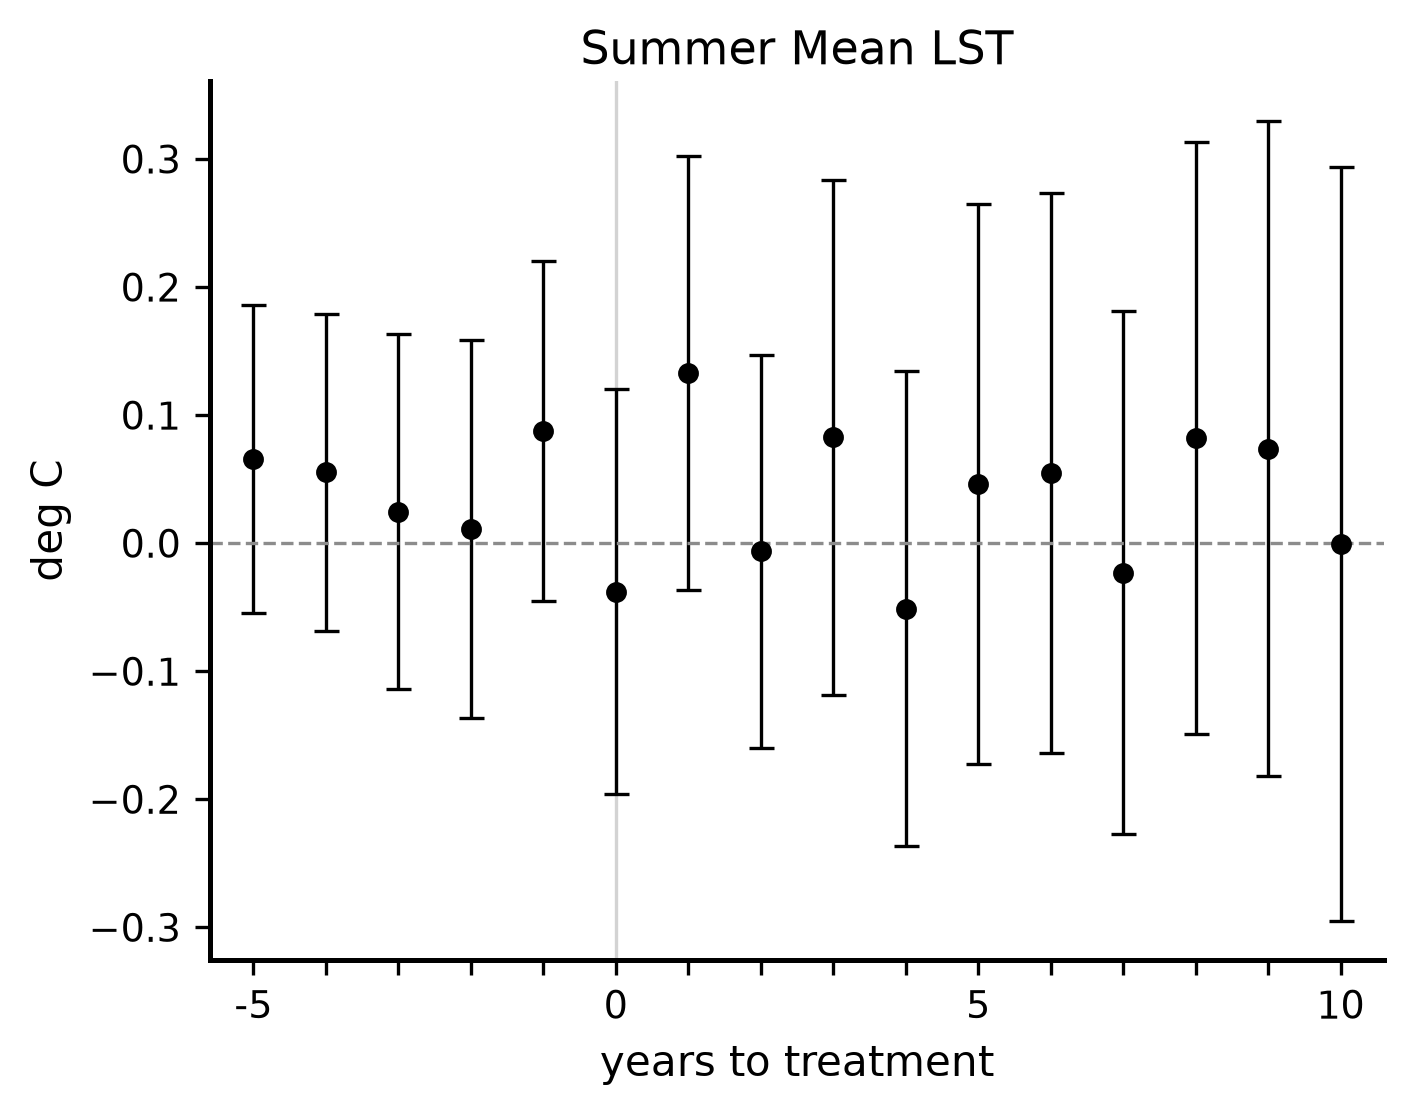
\includegraphics[width=0.47\textwidth]{event_study_bjs_dr_lst_summer_mean_20km} &
  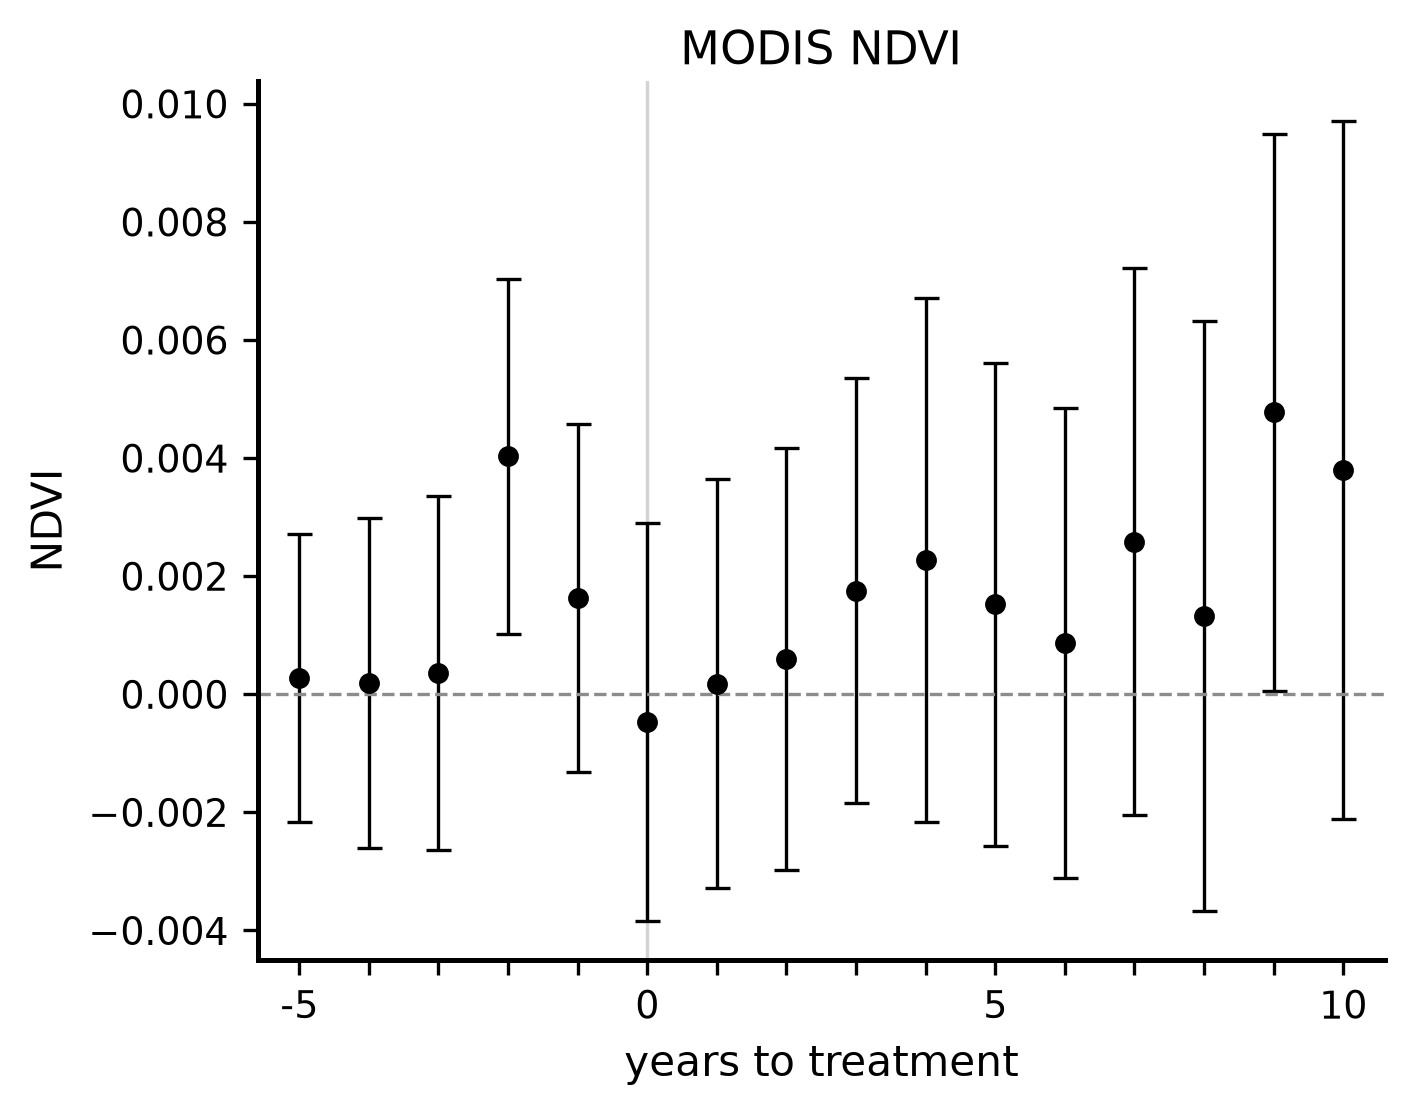
\includegraphics[width=0.47\textwidth]{event_study_bjs_dr_ndvi_mean_20km} \\[2pt]
  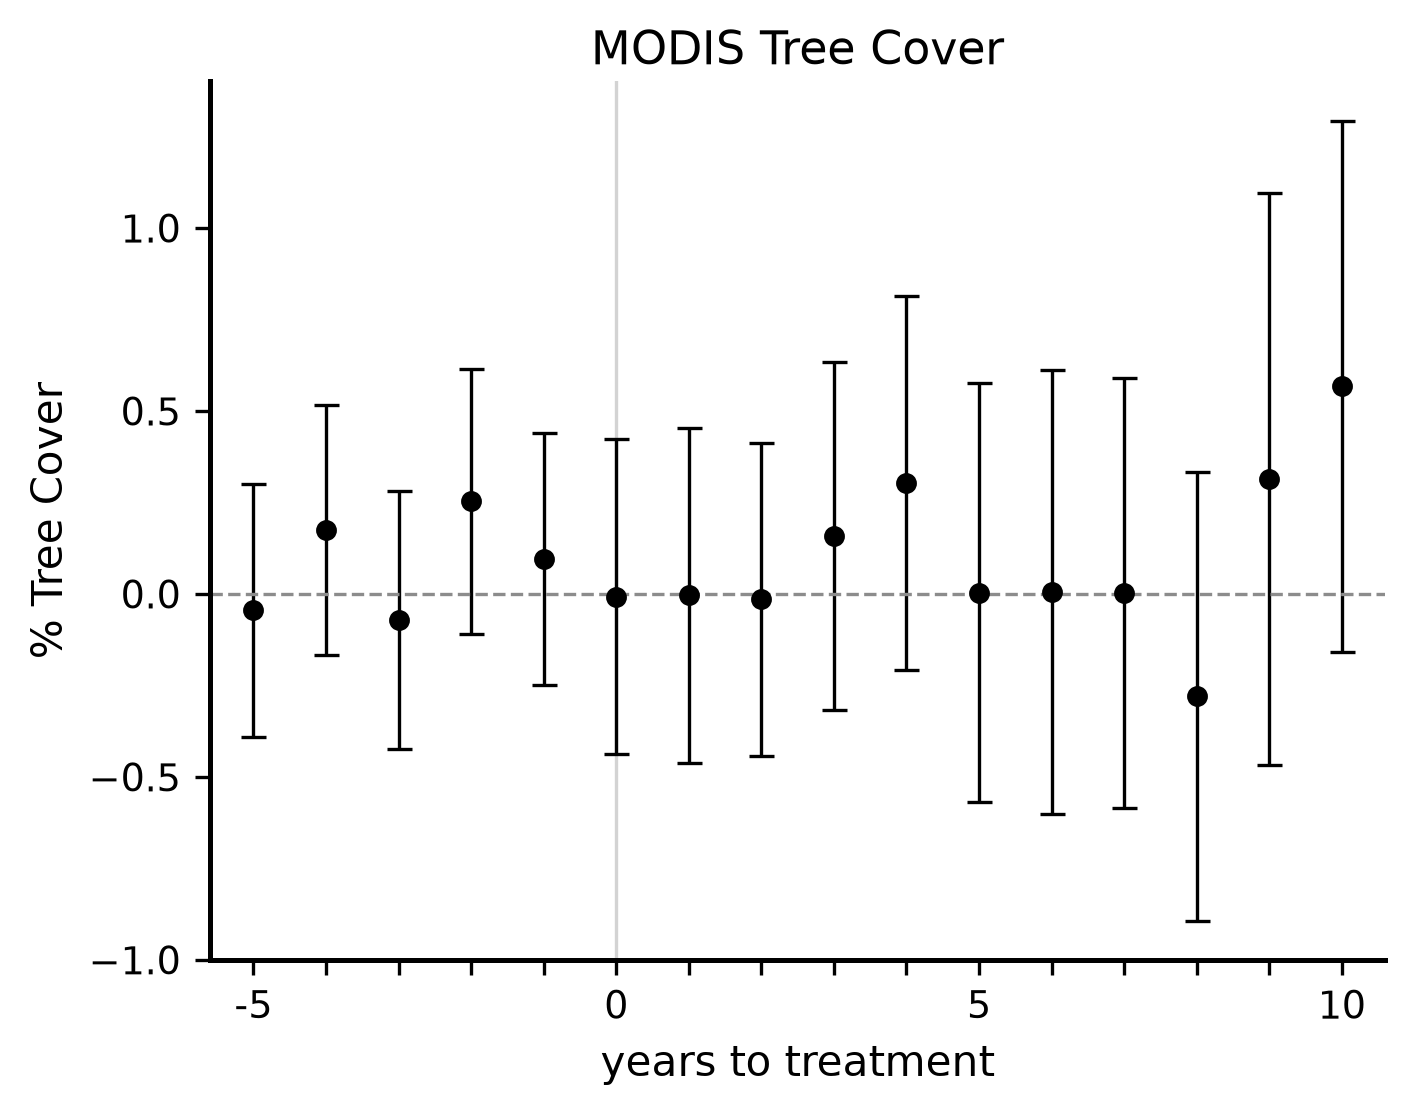
\includegraphics[width=0.47\textwidth]{event_study_bjs_dr_tree_cover_mean_20km} &
  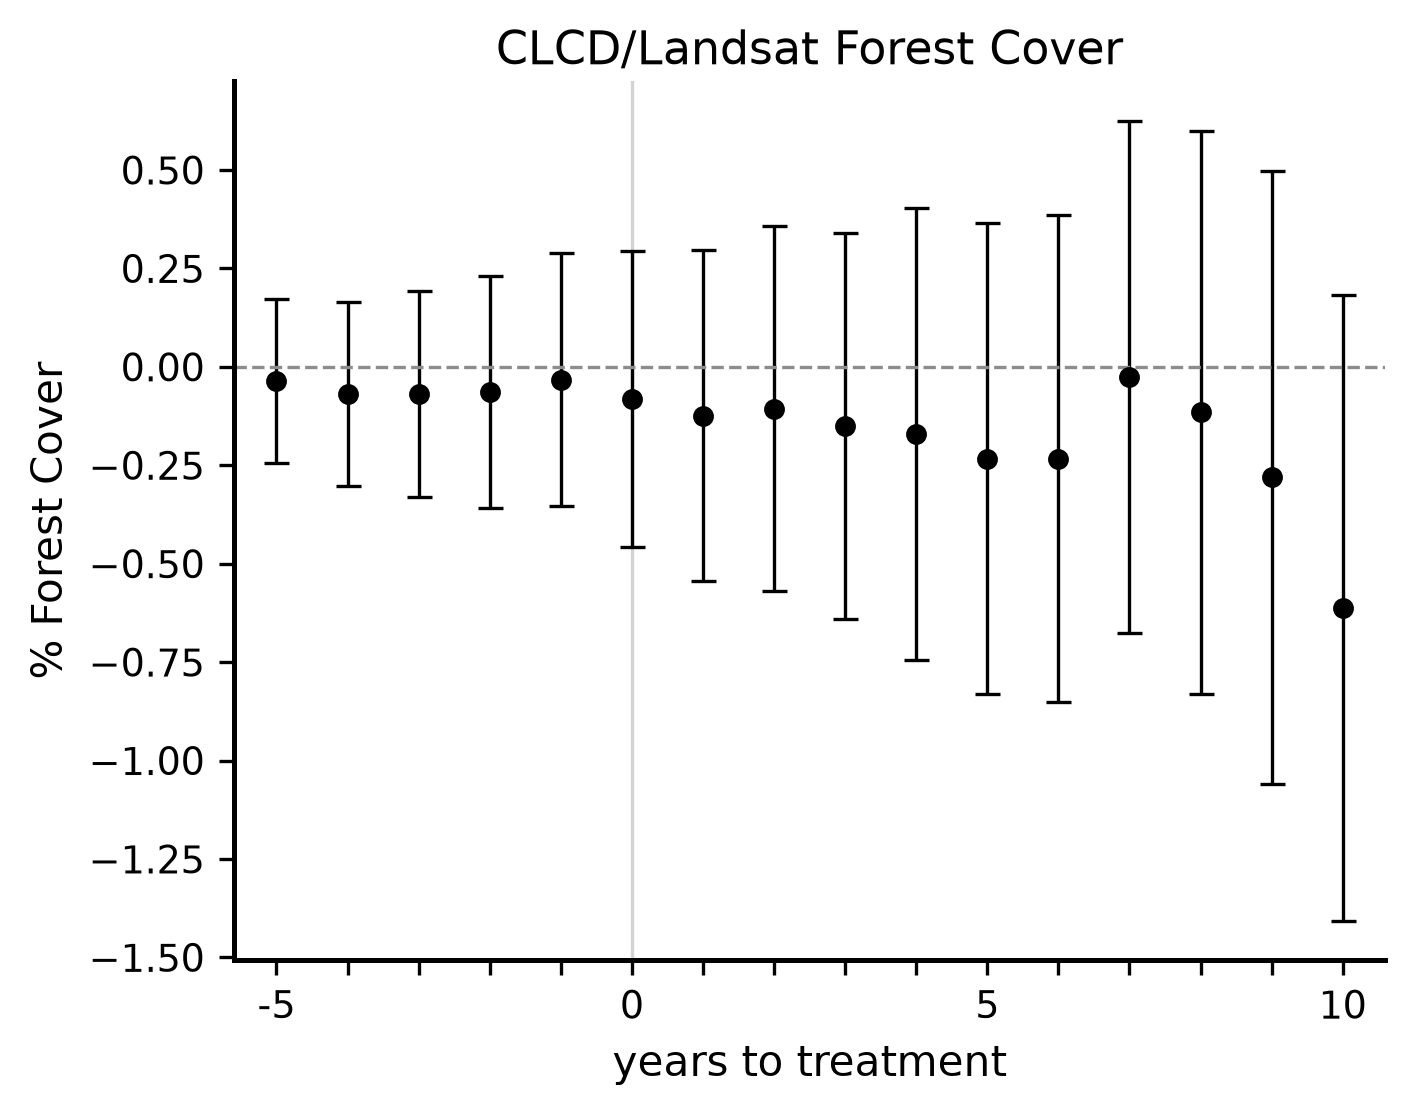
\includegraphics[width=0.47\textwidth]{event_study_bjs_dr_clcd_forest_pct_20km}
\end{tabular}
\end{singlespace}
\caption{BJS imputation with covariate adjustment (BJS with controls) event
studies for outcomes averaged over pixels within 20~km of the city centroid,
corresponding to column~(1) of Table~\ref{tab:att}.  The horizontal axis
shows years to treatment ($t = 0$ is the designation year, $t = -1$ is the
reference period).  Dots are point estimates; vertical whiskers show the
95\% confidence interval clustered at the city level.
\textit{LST ($^\circ$C)}: top left.
\textit{NDVI (index)}: top right.
\textit{Tree cover (\%)}: bottom left.
\textit{CLCD forest (pp)}: bottom right.}
\label{fig:main}
\end{figure}


Appendix Figures~\ref{fig:bjs_5km}, \ref{fig:cs_dr},  \ref{fig:cs_pref}, and~\ref{fig:station_bjs} present event study figures like those in figure \ref{fig:main}, but for columns 2, 3, 5, and 6, respectively. Each tells more or less the same story. Pre-period and post period estimates are imprecisely estimated and scattered around zero. The CLCD event study in the bottom right of figures \ref{fig:bjs_5km} and \ref{fig:cs_dr} which show that treatment with NFCP designation may have decreased forest cover.  That \ref{fig:bjs_5km} also suggests a decreasing pretrend invites the conjecture that cities with decreasing central forest cover selected into the program and continued on this trend after designation.  None of the event studies in any of the figures offers any support to the \cite{Ma2026} claim that NFCP designation caused a reduction in urban temperature or increased forest cover.

% ------------------------------------------------------------------
\section{Conclusion}
\label{sec:conclusion}
% ------------------------------------------------------------------

The temperature effect of NFCP designation is not robustly identified under
any of the heterogeneity robust estimators that we consider.
BJS with controls gives $+0.032^\circ$C ($SE = 0.106$) at 20~km, DR gives
$+0.016^\circ$C ($SE = 0.097$), and CS gives $+0.067^\circ$C ($SE = 0.095$).
Across all three specifications the temperature estimates are slightly positve, statistically insignificant, and allow us to rule anything except a small cooling effect. The \citet{Ma2026} temperature result does not appear in our analyses.

The vegetation results add an independent argument against the proposed
mechanism.  MODIS NDVI, MODIS tree cover, and CLCD forest cover show no
post-designation increase at any buffer radius.  CLCD forest share declines
marginally at 5~km: BJS with controls gives $-0.585$ pp ($p < 0.10$,
column~2).  Without a greening signal at any radius, there is no plausible
mechanism by which the NFCP could reduce urban heat.

We conclude that the main result in \citet{Ma2026} is not robustly identified.  
% ------------------------------------------------------------------
\section*{Data and Code Availability}

MODIS land surface temperature (MOD11A2), NDVI (MOD13A3), and tree cover
(MOD44B) are publicly available from NASA EOSDIS.
The China Land Cover Dataset (CLCD) is publicly available from Zenodo
(record~18180184; \citealt{Yang2021}).
GHCN-Daily station temperature records are publicly available from NOAA
\citep{Menne2012}.
NFCP designation lists are publicly available from the National Forestry
and Grassland Administration of China.
Estimation code is available from the author upon request.

% ------------------------------------------------------------------
\bibliographystyle{plainnat}
\bibliography{refs}

% ------------------------------------------------------------------
\appendix
\setcounter{figure}{0}
\renewcommand{\thefigure}{A\arabic{figure}}
\setcounter{table}{0}
\renewcommand{\thetable}{A\arabic{table}}
\FloatBarrier

\pagebreak
\section*{Appendix}

Figure~\ref{fig:bjs_5km} shows BJS with controls event studies at the 5~km
buffer, corresponding to column~(2) of Table~\ref{tab:att}.  All estimates
are consistent with the 20~km null in Figure~\ref{fig:main}.

\begin{figure}[h]
\centering
\begin{singlespace}
\begin{tabular}{@{}cc@{}}
  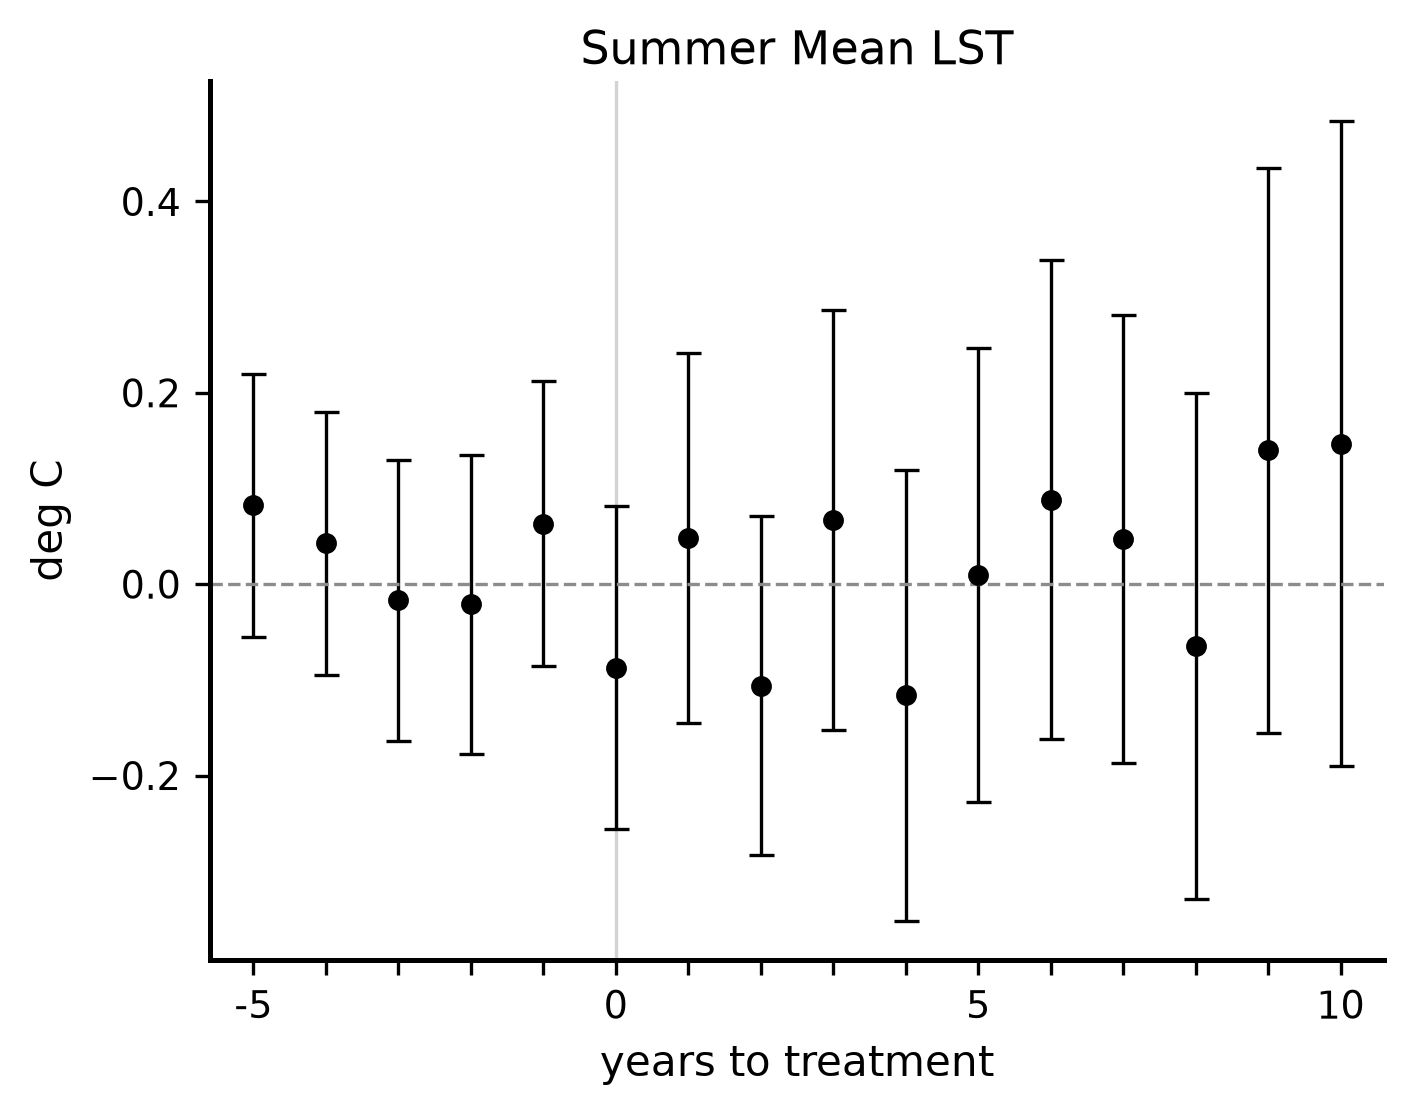
\includegraphics[width=0.47\textwidth]{event_study_bjs_dr_lst_summer_mean_5km} &
  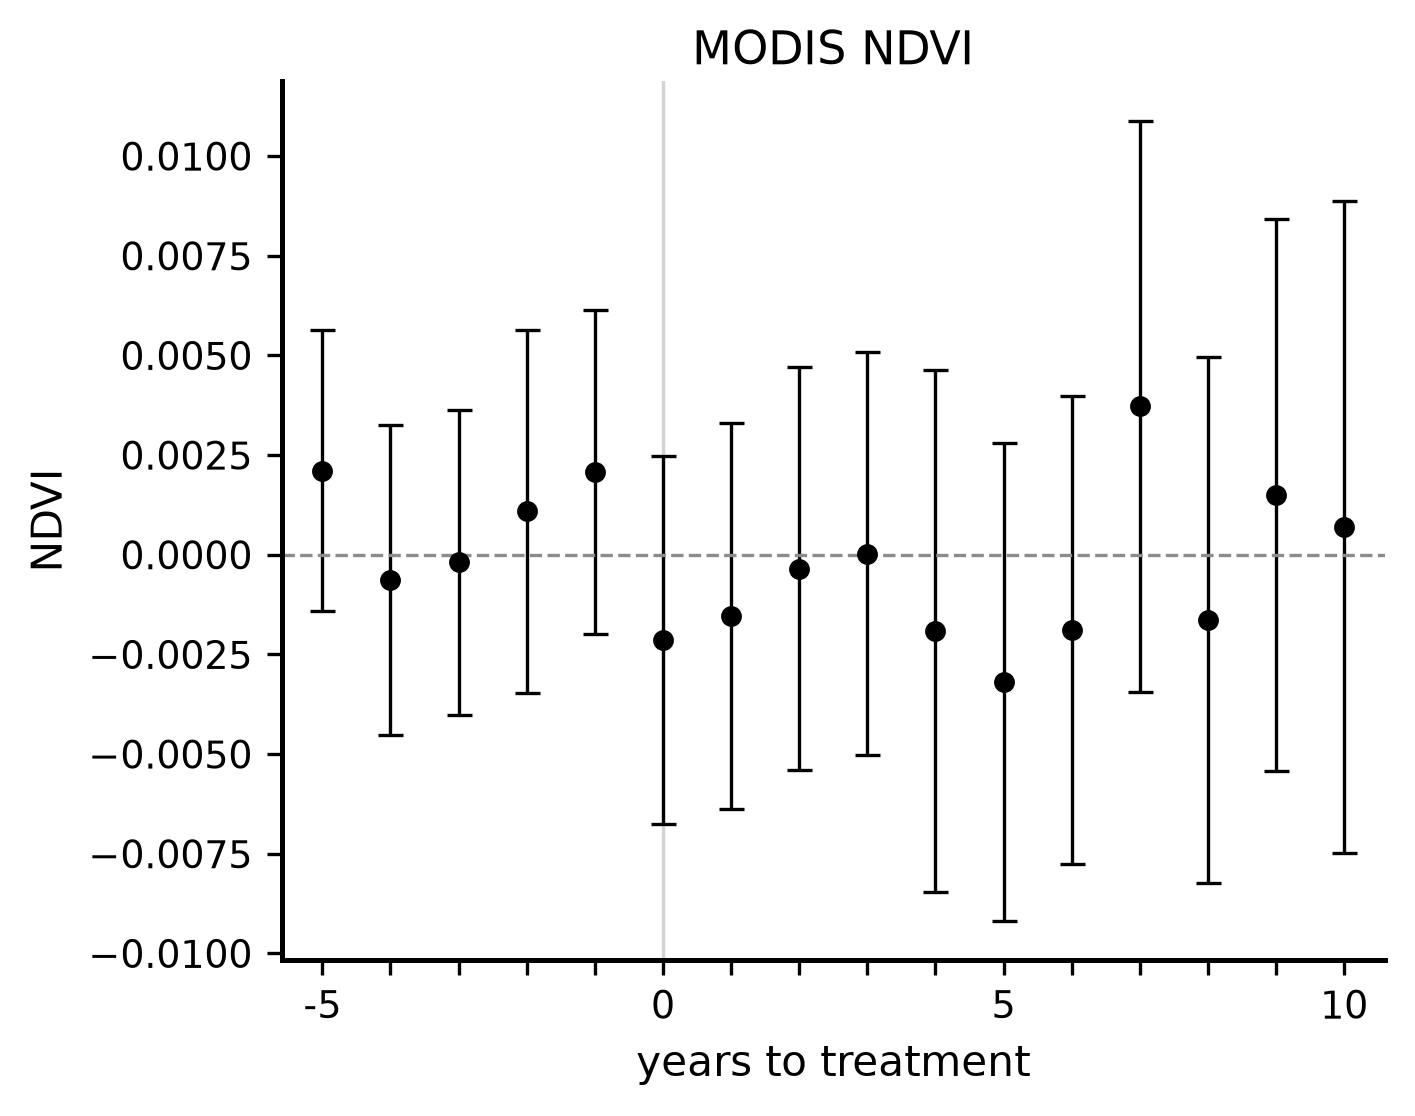
\includegraphics[width=0.47\textwidth]{event_study_bjs_dr_ndvi_mean_5km} \\[2pt]
  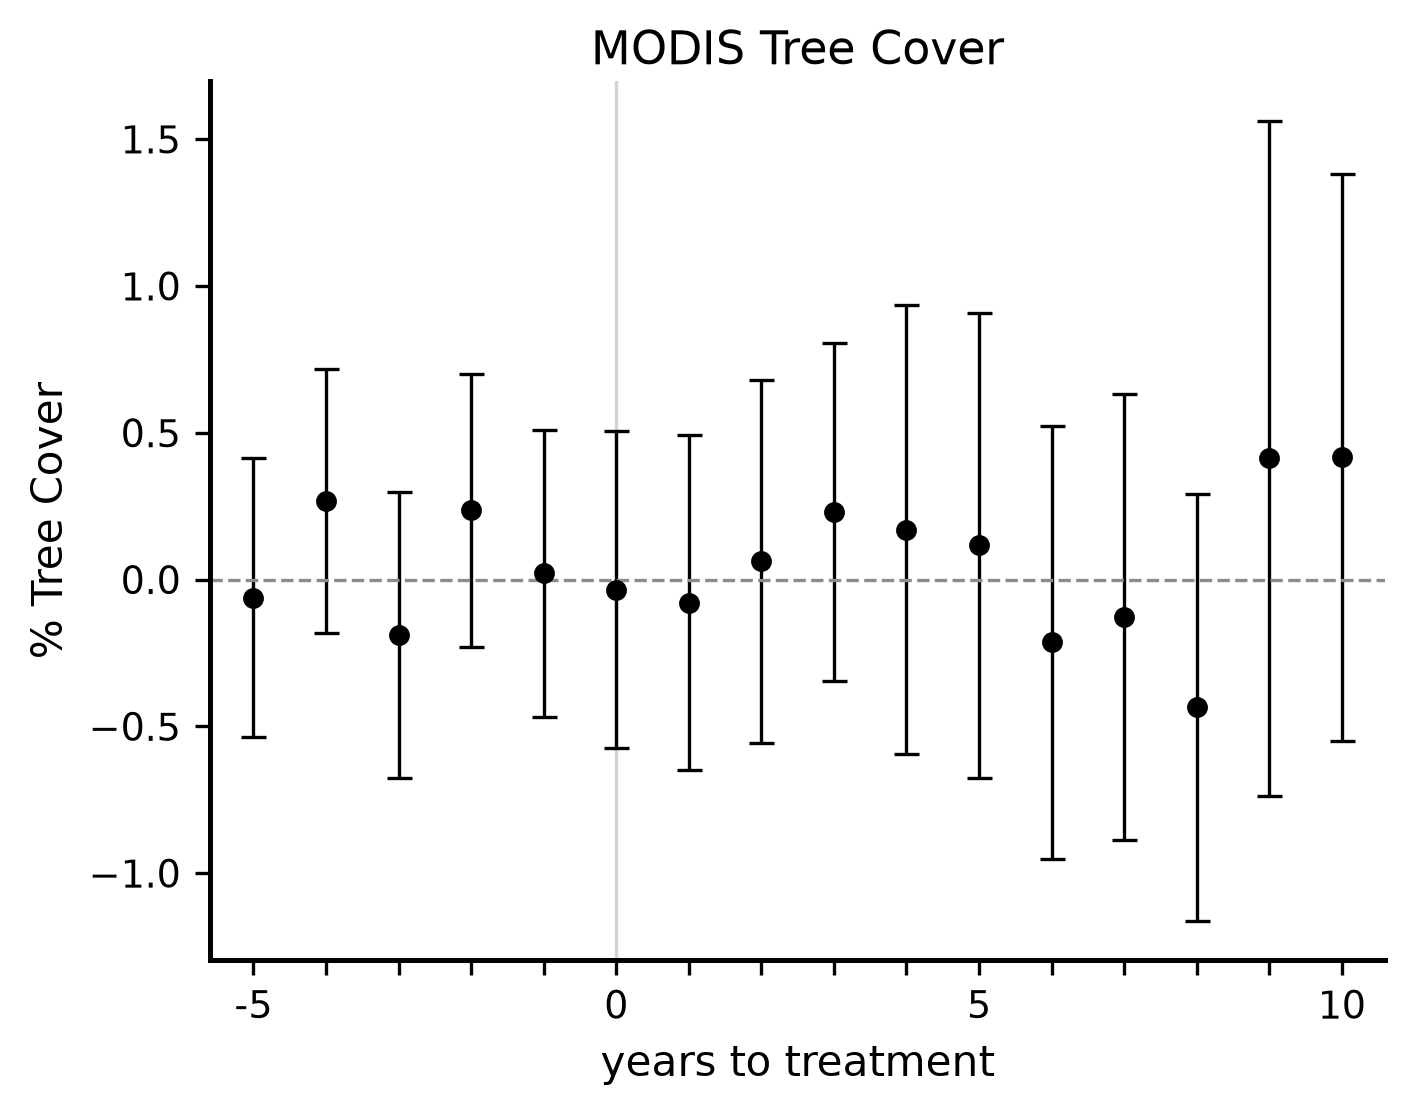
\includegraphics[width=0.47\textwidth]{event_study_bjs_dr_tree_cover_mean_5km} &
  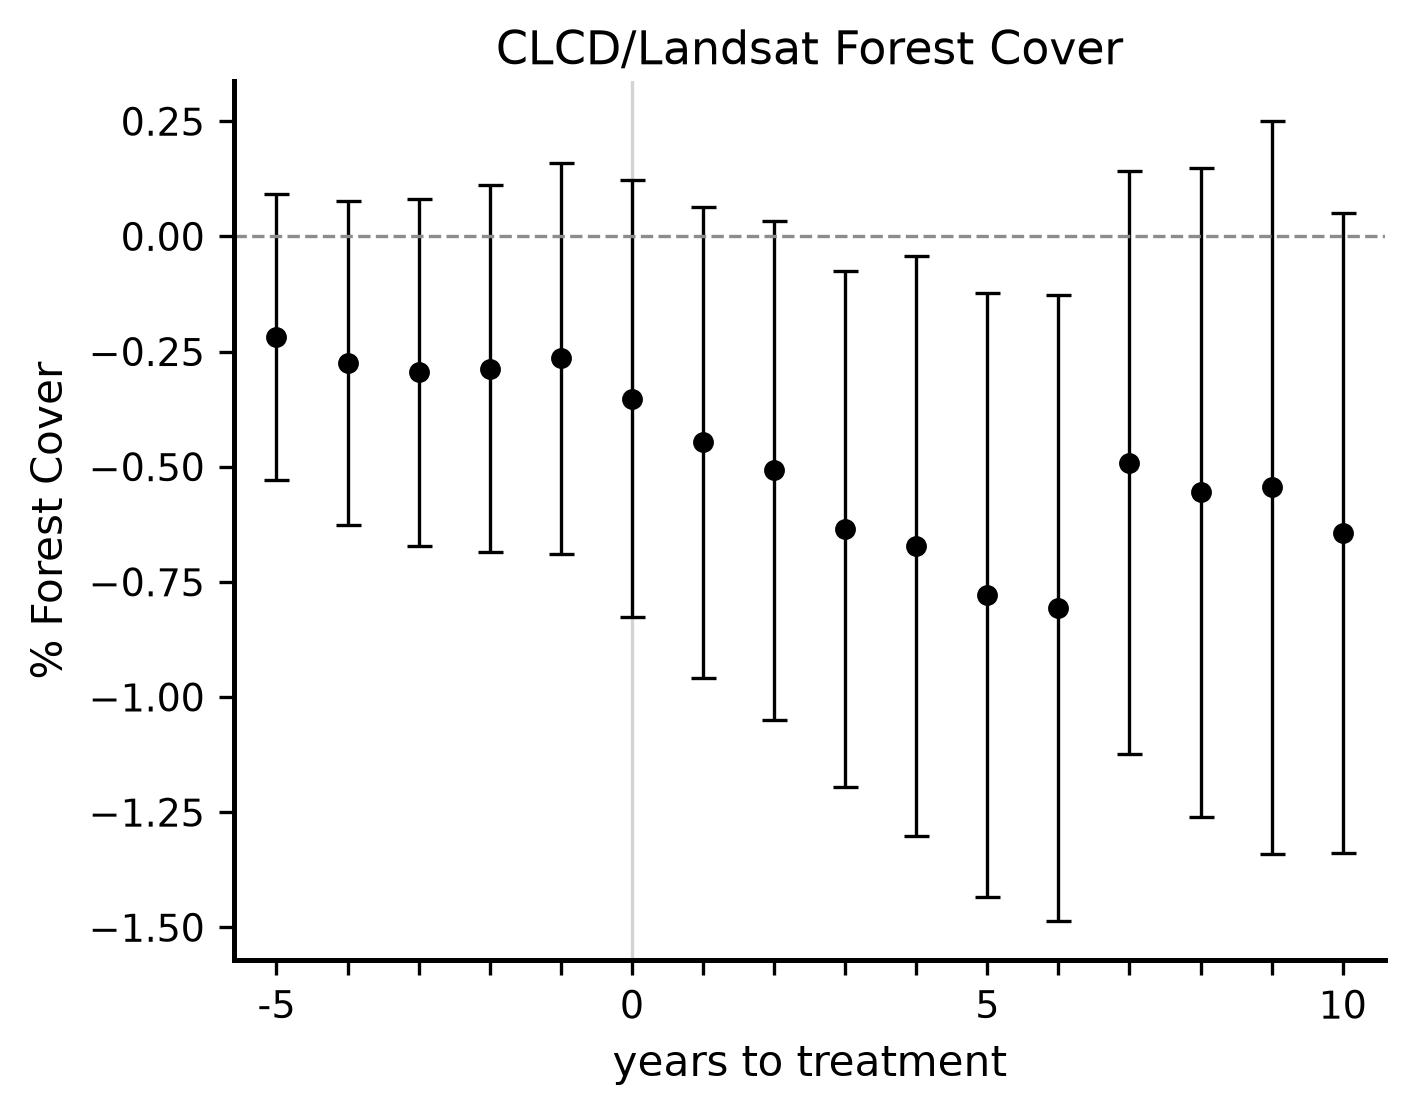
\includegraphics[width=0.47\textwidth]{event_study_bjs_dr_clcd_forest_pct_5km}
\end{tabular}
\end{singlespace}
\caption{BJS imputation with covariate adjustment (BJS with controls) event
studies at the 5~km buffer, corresponding to column~(2) of
Table~\ref{tab:att}.  The horizontal axis shows years to treatment ($t = 0$
is the designation year, $t = -1$ is the reference period).  Dots are point
estimates; vertical whiskers show the 95\% confidence interval clustered at
the city level.
\textit{LST ($^\circ$C)}: top left.
\textit{NDVI (index)}: top right.
\textit{Tree cover (\%)}: bottom left.
\textit{CLCD forest (pp)}: bottom right.}
\label{fig:bjs_5km}
\end{figure}

Figure~\ref{fig:cs_dr} shows DR event studies at 20~km, corresponding to
column~(3) of Table~\ref{tab:att}.  Pre-designation coefficients are near
zero and individually insignificant, confirming that conditional parallel
trends hold under covariate adjustment.

\begin{figure}[h]
\centering
\begin{singlespace}
\begin{tabular}{@{}cc@{}}
  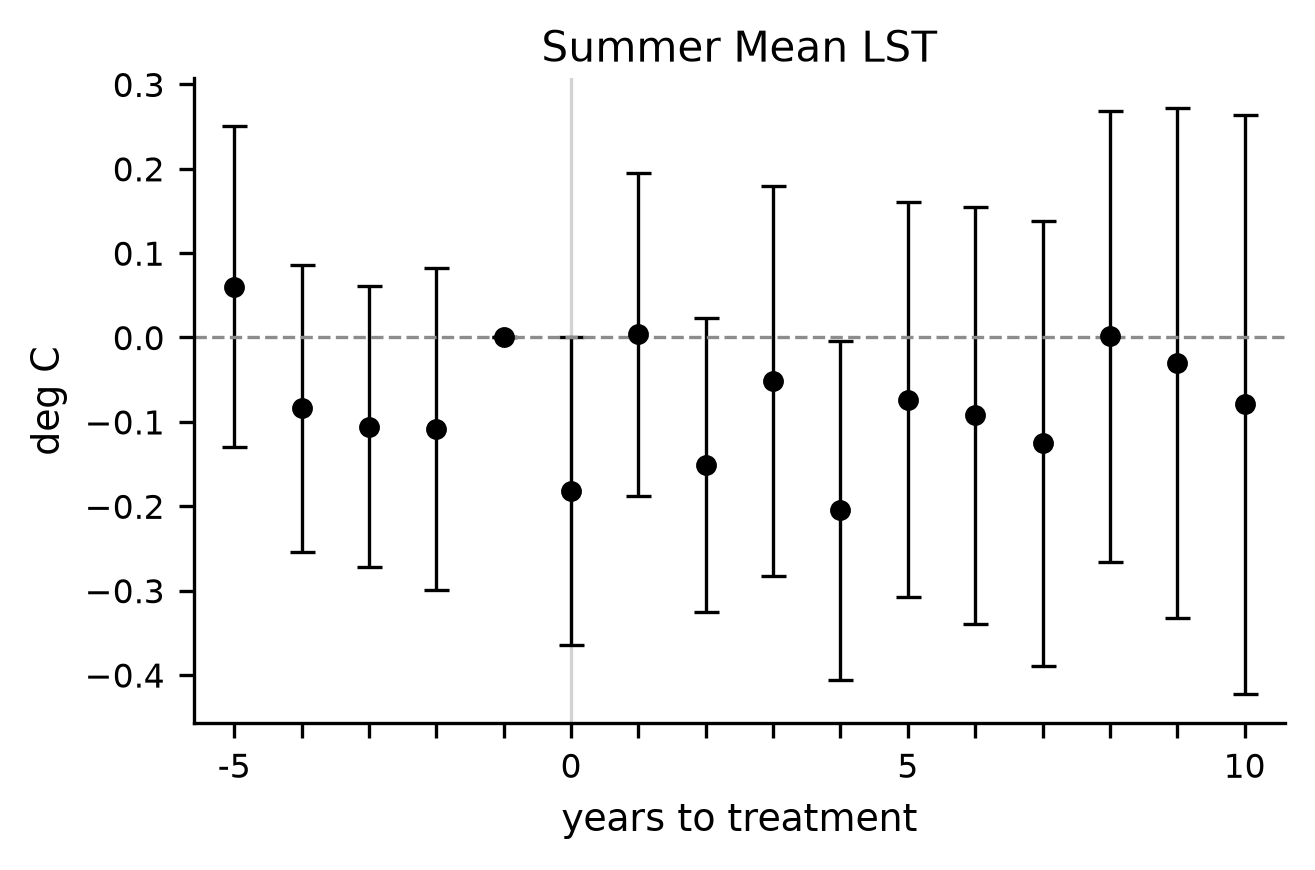
\includegraphics[width=0.47\textwidth]{stata/city_lst_summer_mean_20km_cs_dr} &
  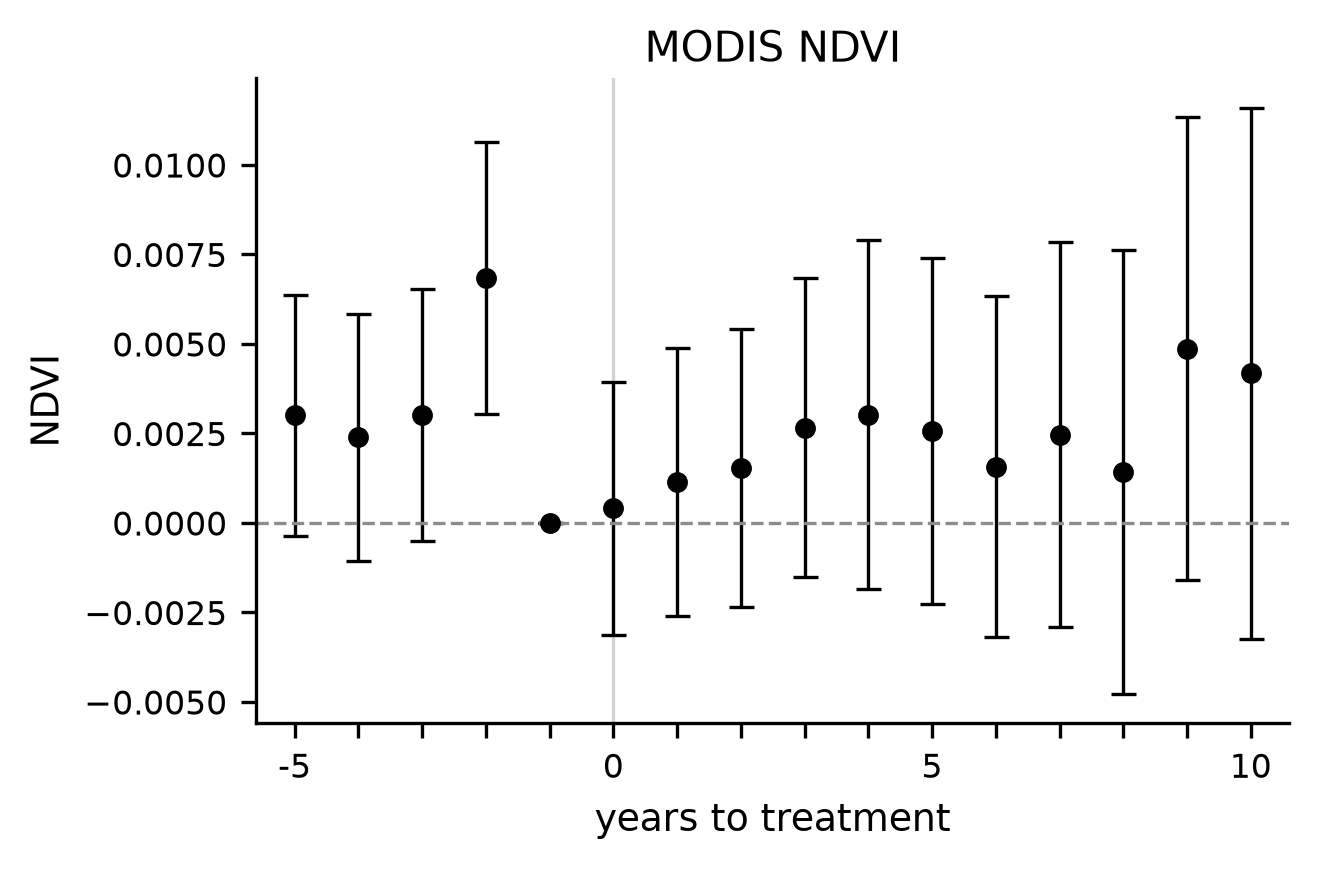
\includegraphics[width=0.47\textwidth]{stata/city_ndvi_mean_20km_cs_dr} \\[2pt]
  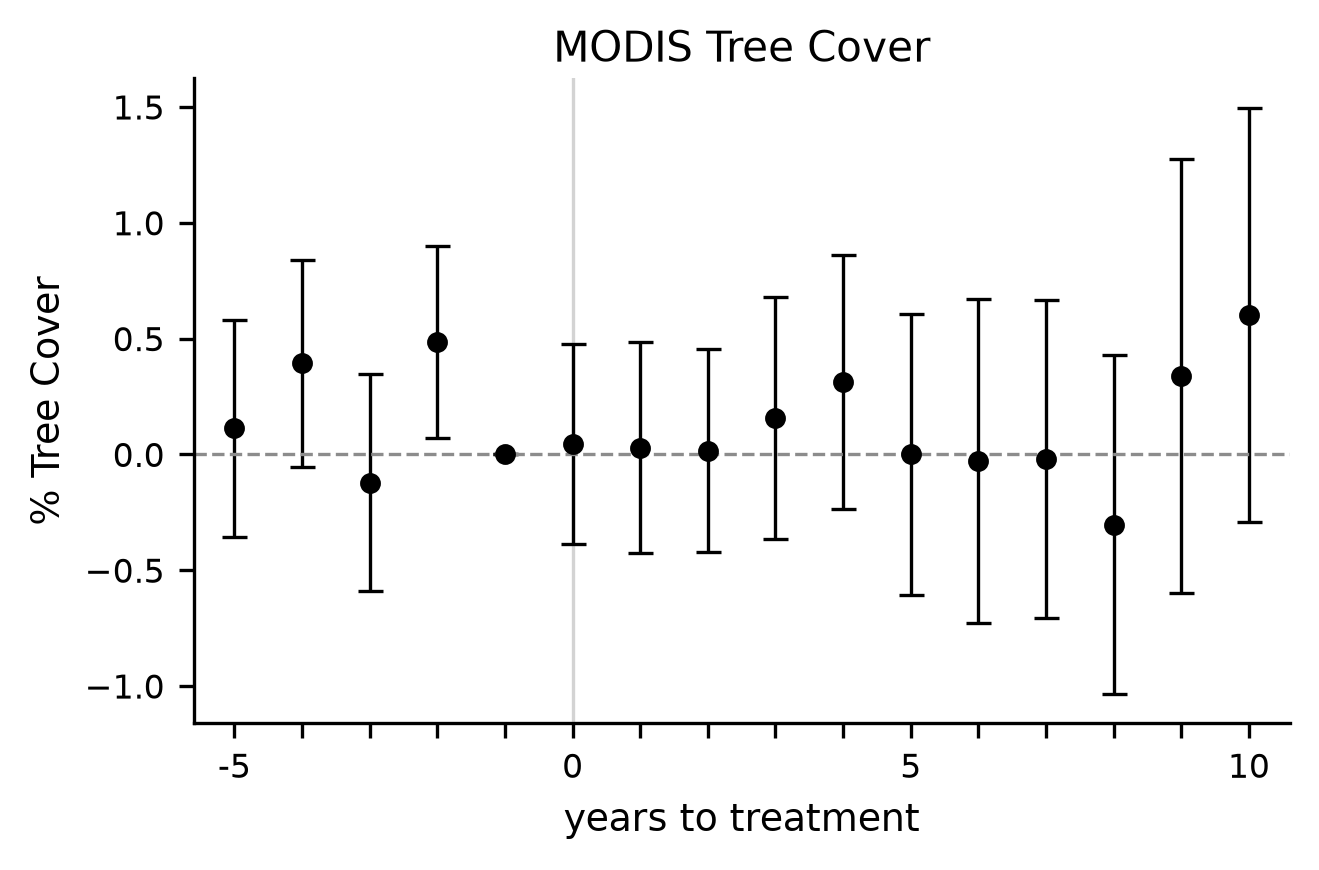
\includegraphics[width=0.47\textwidth]{stata/city_tree_cover_mean_20km_cs_dr} &
  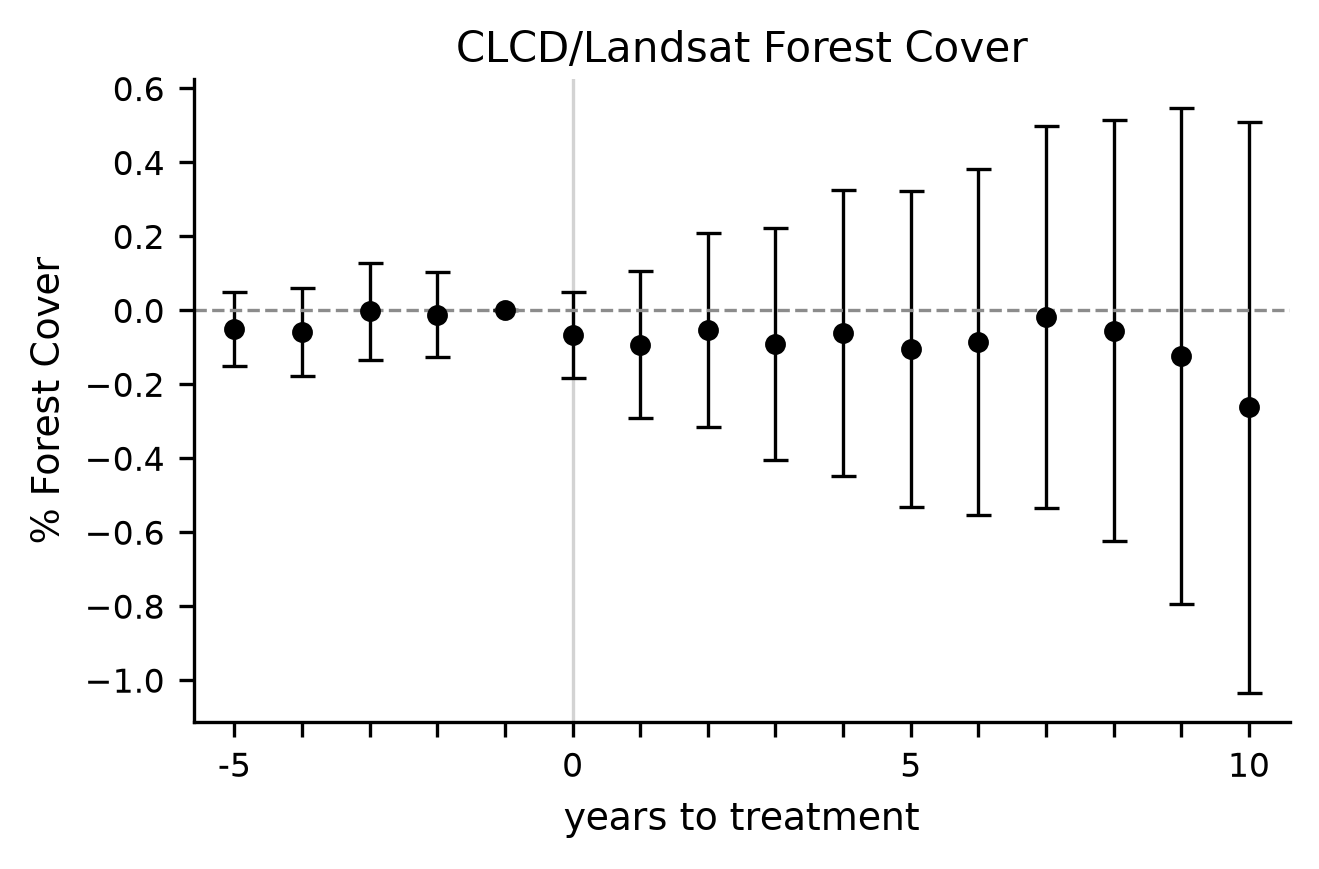
\includegraphics[width=0.47\textwidth]{stata/city_clcd_forest_pct_20km_cs_dr}
\end{tabular}
\end{singlespace}
\caption{Doubly robust Callaway--Sant'Anna (DR) event studies at 20~km
conditioning on pre-determined city characteristics (latitude, longitude, and
log pre-treatment population), corresponding to column~(3) of
Table~\ref{tab:att}.  The horizontal axis shows years to treatment ($t = 0$
is the designation year, $t = -1$ is the reference period).  Dots are point
estimates; vertical whiskers show the 95\% confidence interval from Stata's
\texttt{csdid} \citep{CS2021, SantAnnaZhao2020}.
\textit{LST ($^\circ$C)}: top left.
\textit{NDVI (index)}: top right.
\textit{Tree cover (\%)}: bottom left.
\textit{CLCD forest (pp)}: bottom right.}
\label{fig:cs_dr}
\end{figure}

Figure~\ref{fig:cs_pref} shows CS event studies at the prefecture-level
geography, corresponding to column~(5) of Table~\ref{tab:att}.  Results
are consistent with the circular-buffer null.

\begin{figure}[h]
\centering
\begin{singlespace}
\begin{tabular}{@{}cc@{}}
  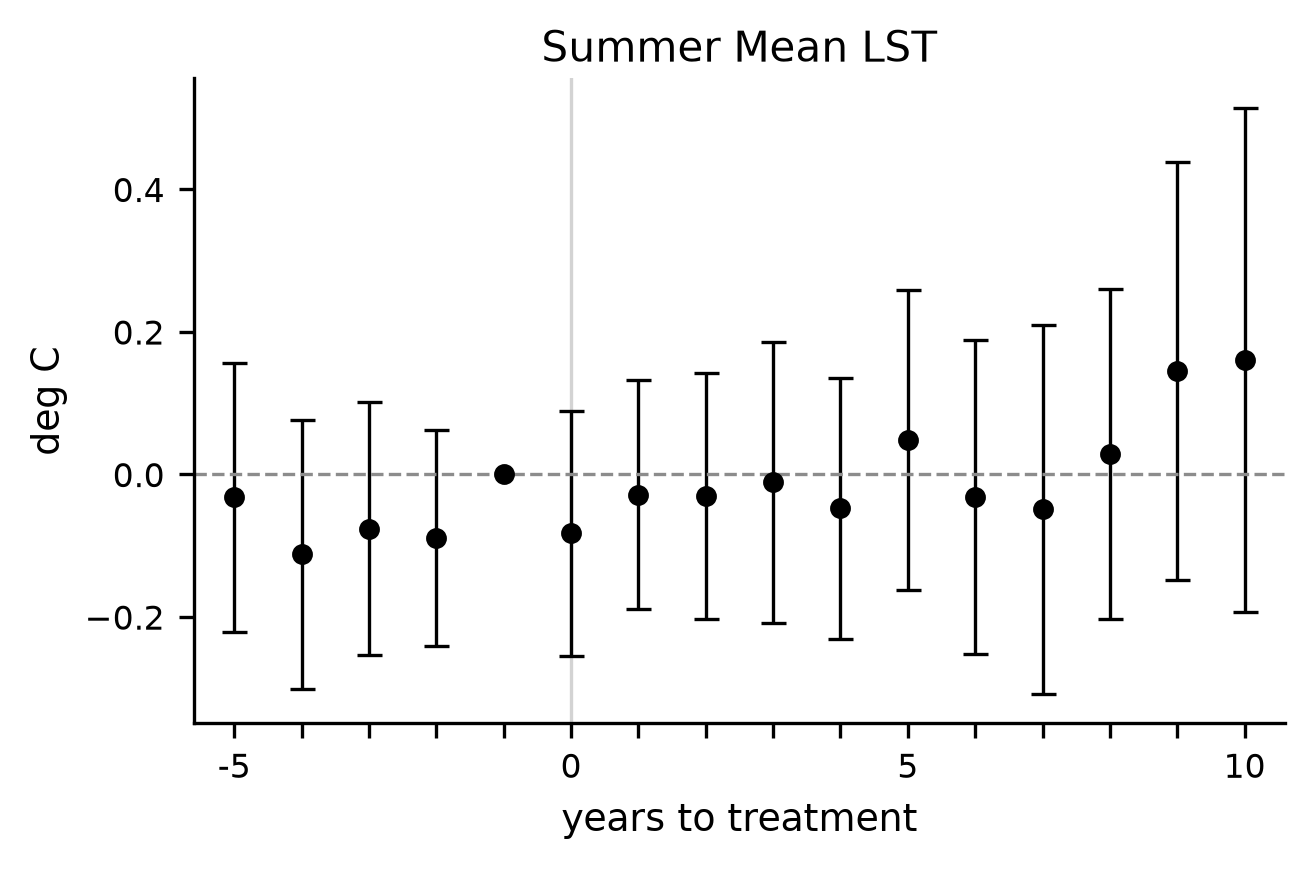
\includegraphics[width=0.47\textwidth]{stata/city_lst_summer_mean_pref_cs} &
  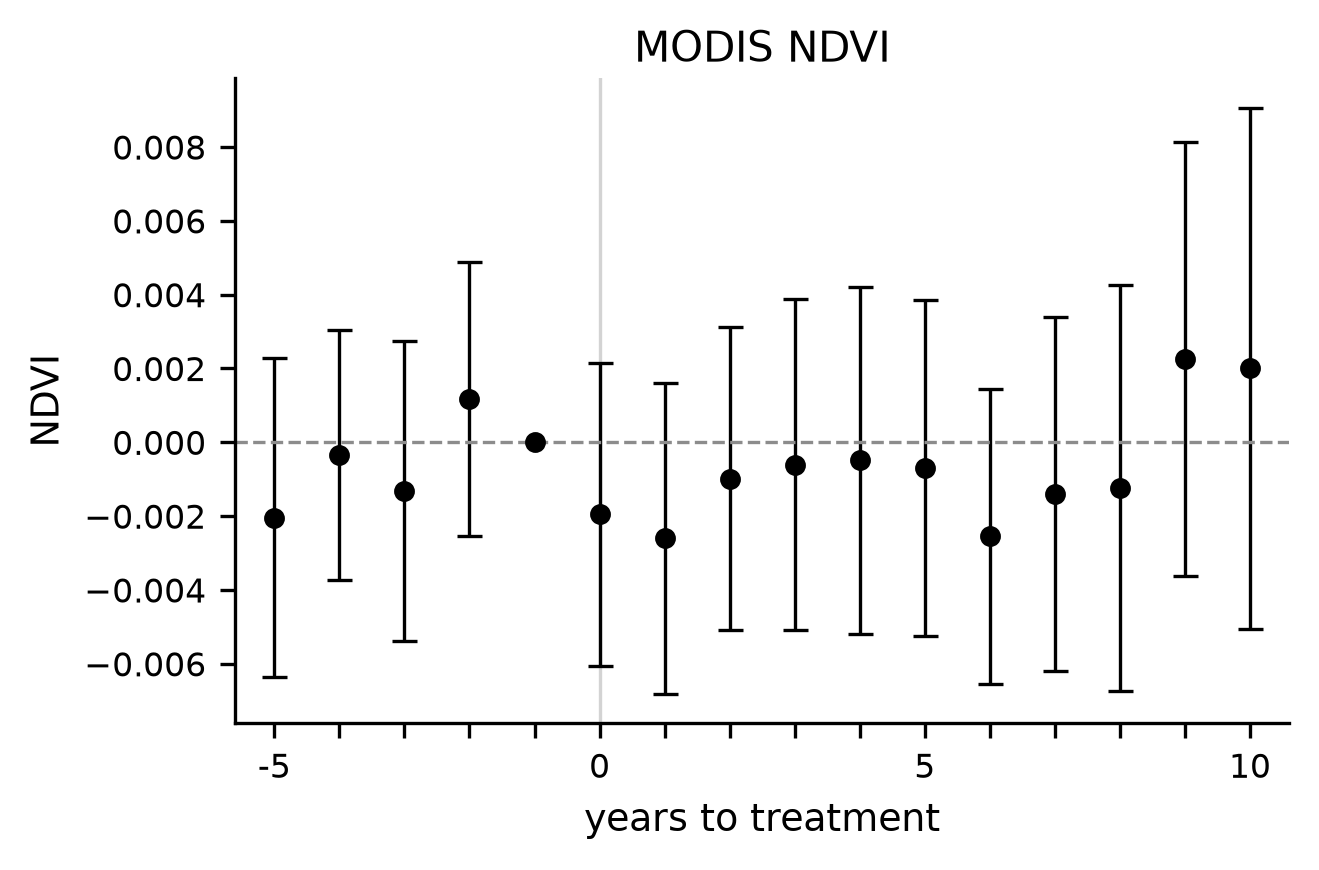
\includegraphics[width=0.47\textwidth]{stata/city_ndvi_mean_pref_cs} \\[2pt]
  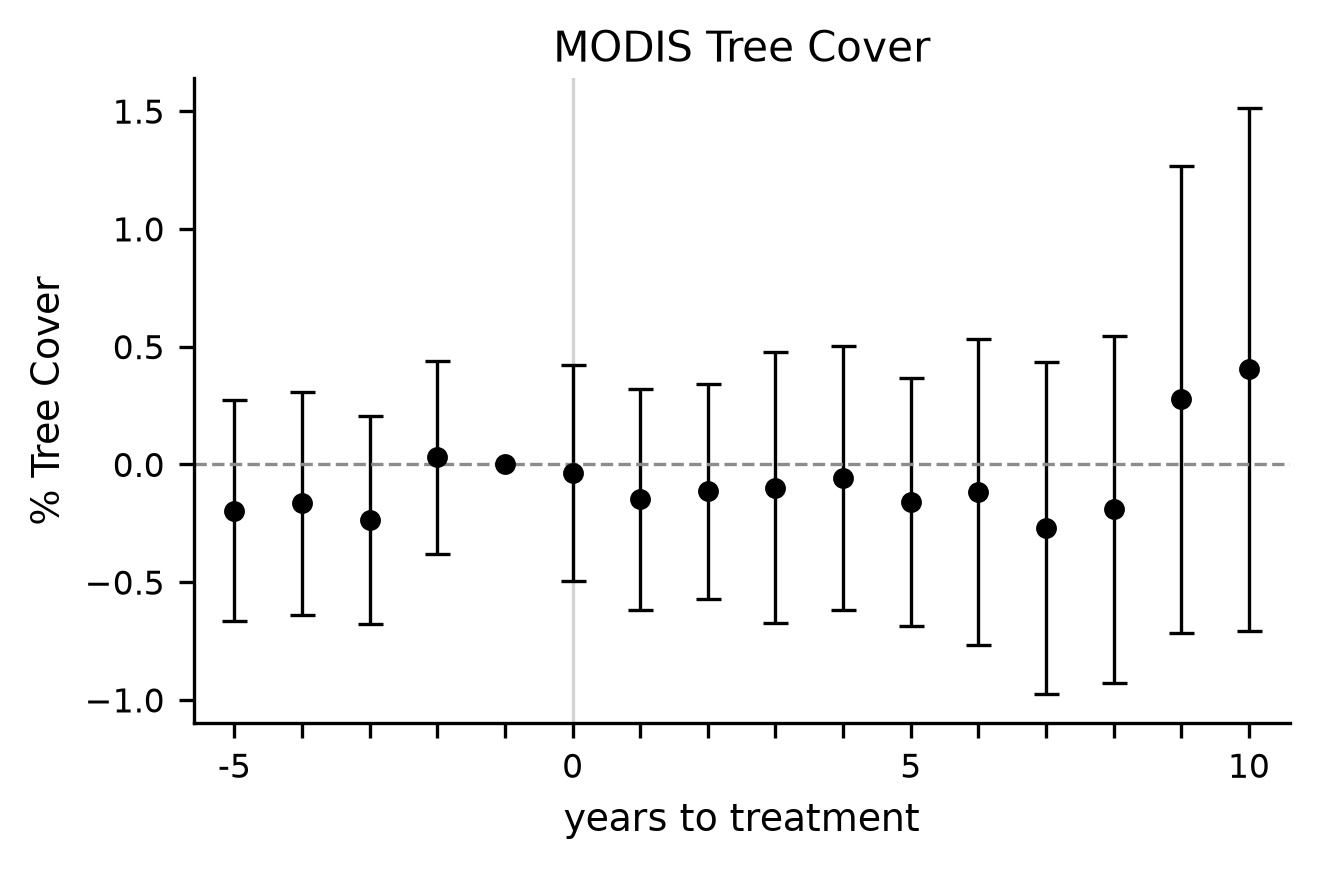
\includegraphics[width=0.47\textwidth]{stata/city_tree_cover_mean_pref_cs} &
  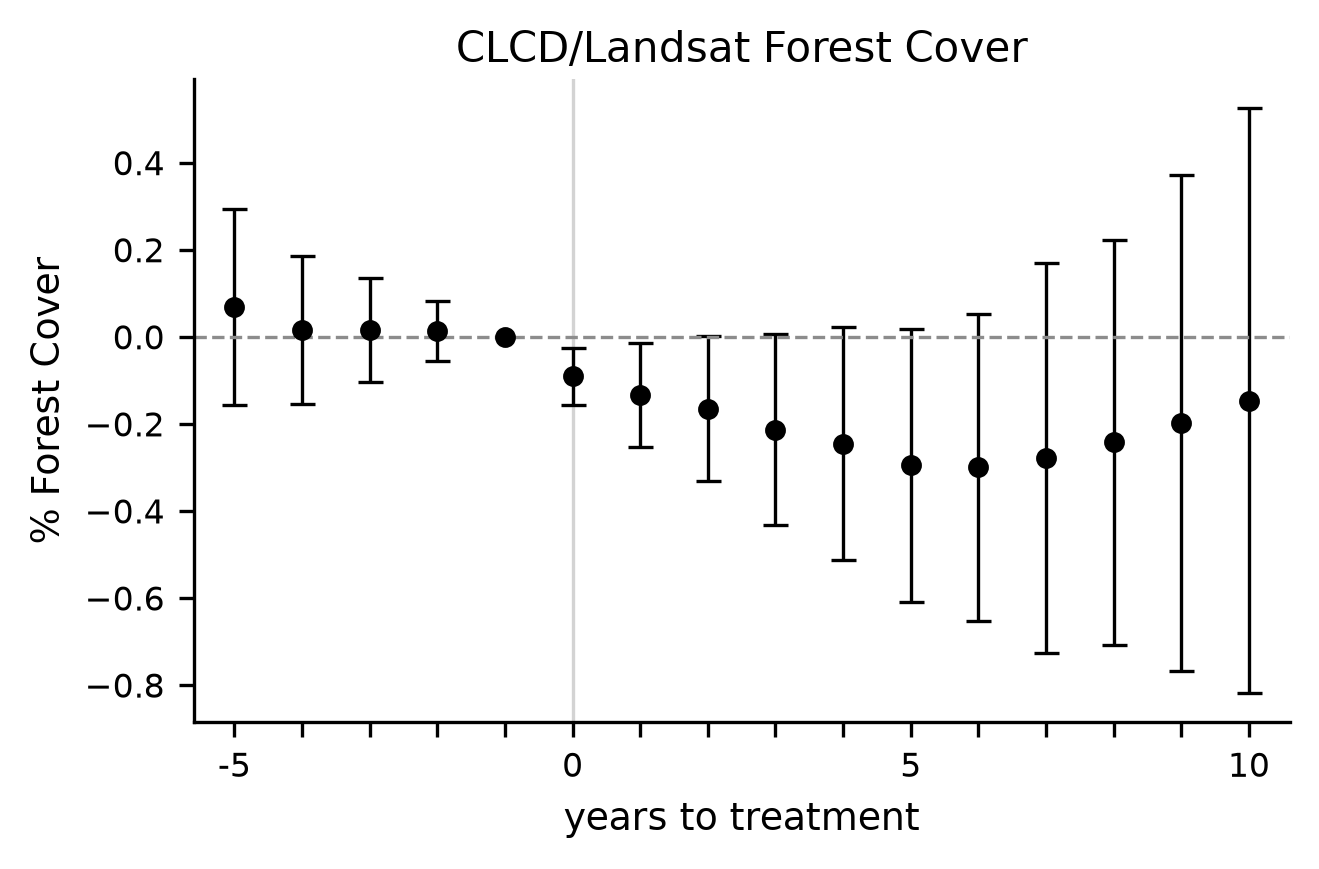
\includegraphics[width=0.47\textwidth]{stata/city_clcd_forest_pct_pref_cs}
\end{tabular}
\end{singlespace}
\caption{Callaway--Sant'Anna (CS, no covariate adjustment) event studies at
the prefecture-level geography, corresponding to column~(5) of
Table~\ref{tab:att}.  The horizontal axis shows years to treatment ($t = 0$
is the designation year, $t = -1$ is the reference period).  Dots are point
estimates; vertical whiskers show the 95\% confidence interval from Stata's
\texttt{csdid} \citep{CS2021}.
\textit{LST ($^\circ$C)}: top left.
\textit{NDVI (index)}: top right.
\textit{Tree cover (\%)}: bottom left.
\textit{CLCD forest (pp)}: bottom right.}
\label{fig:cs_pref}
\end{figure}

Figure~\ref{fig:station_bjs} shows BJS with controls event studies at the
station level, corresponding to column~(6) of Table~\ref{tab:att}.

\begin{figure}[h]
\centering
\begin{singlespace}
\begin{tabular}{@{}cc@{}}
  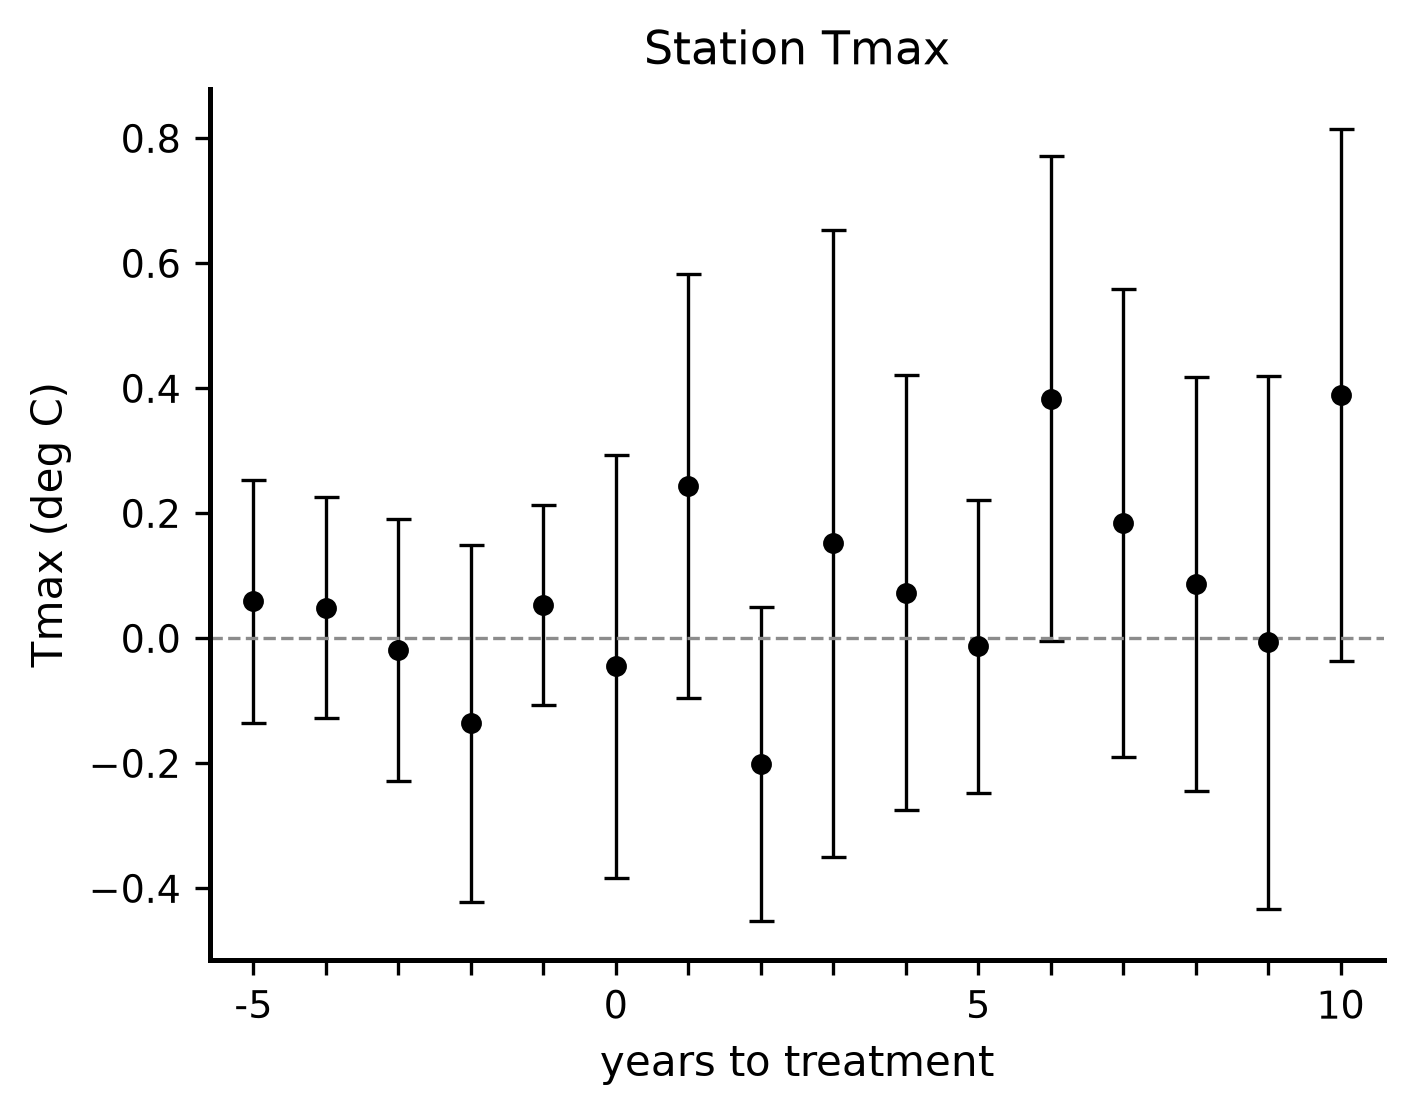
\includegraphics[width=0.47\textwidth]{station_event_study_bjs_dr_tmax-summer-mean} &
  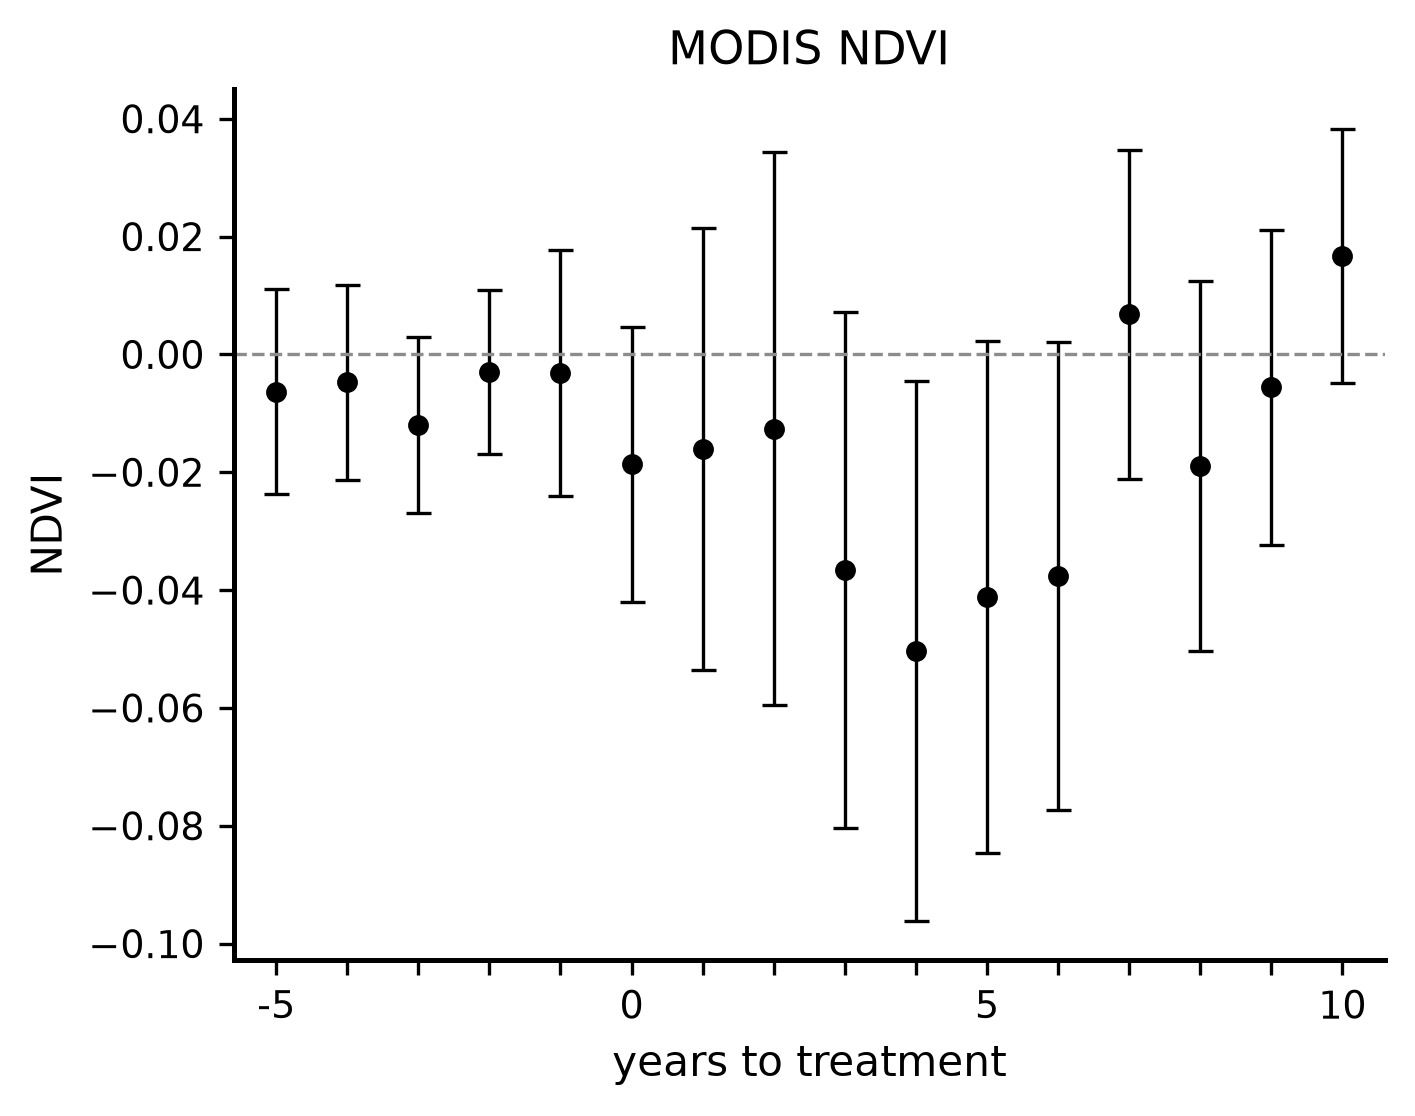
\includegraphics[width=0.47\textwidth]{station_event_study_bjs_dr_ndvi-summer-mean-nearest}\\[4pt]
  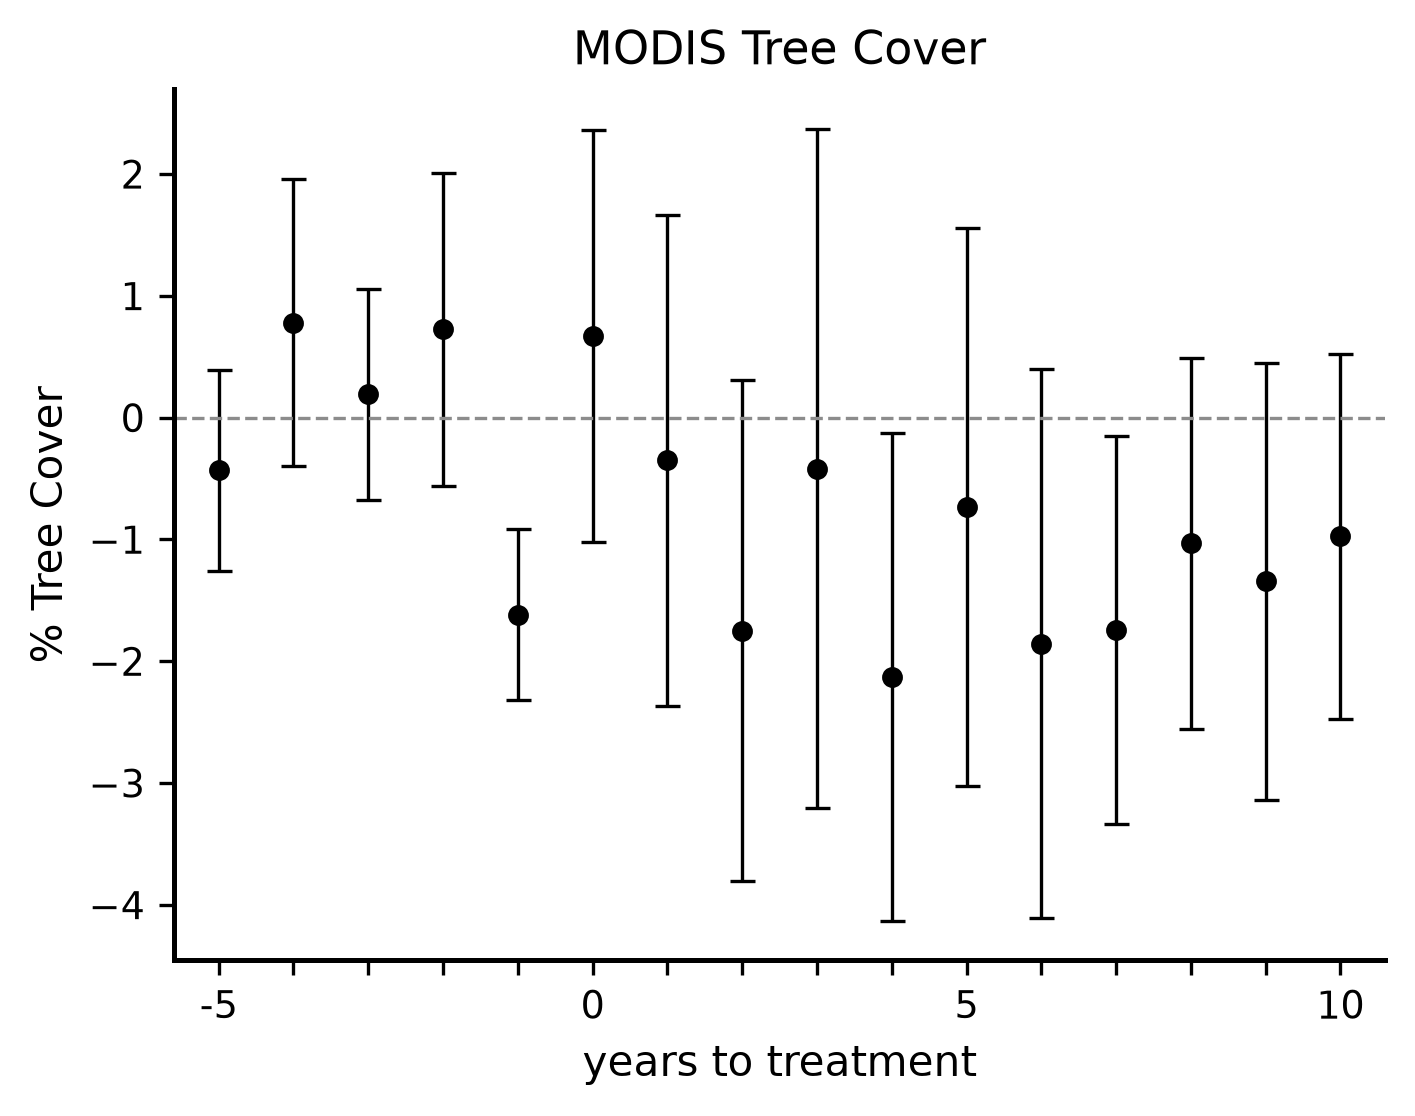
\includegraphics[width=0.47\textwidth]{station_event_study_bjs_dr_tree-cover-nearest} &
  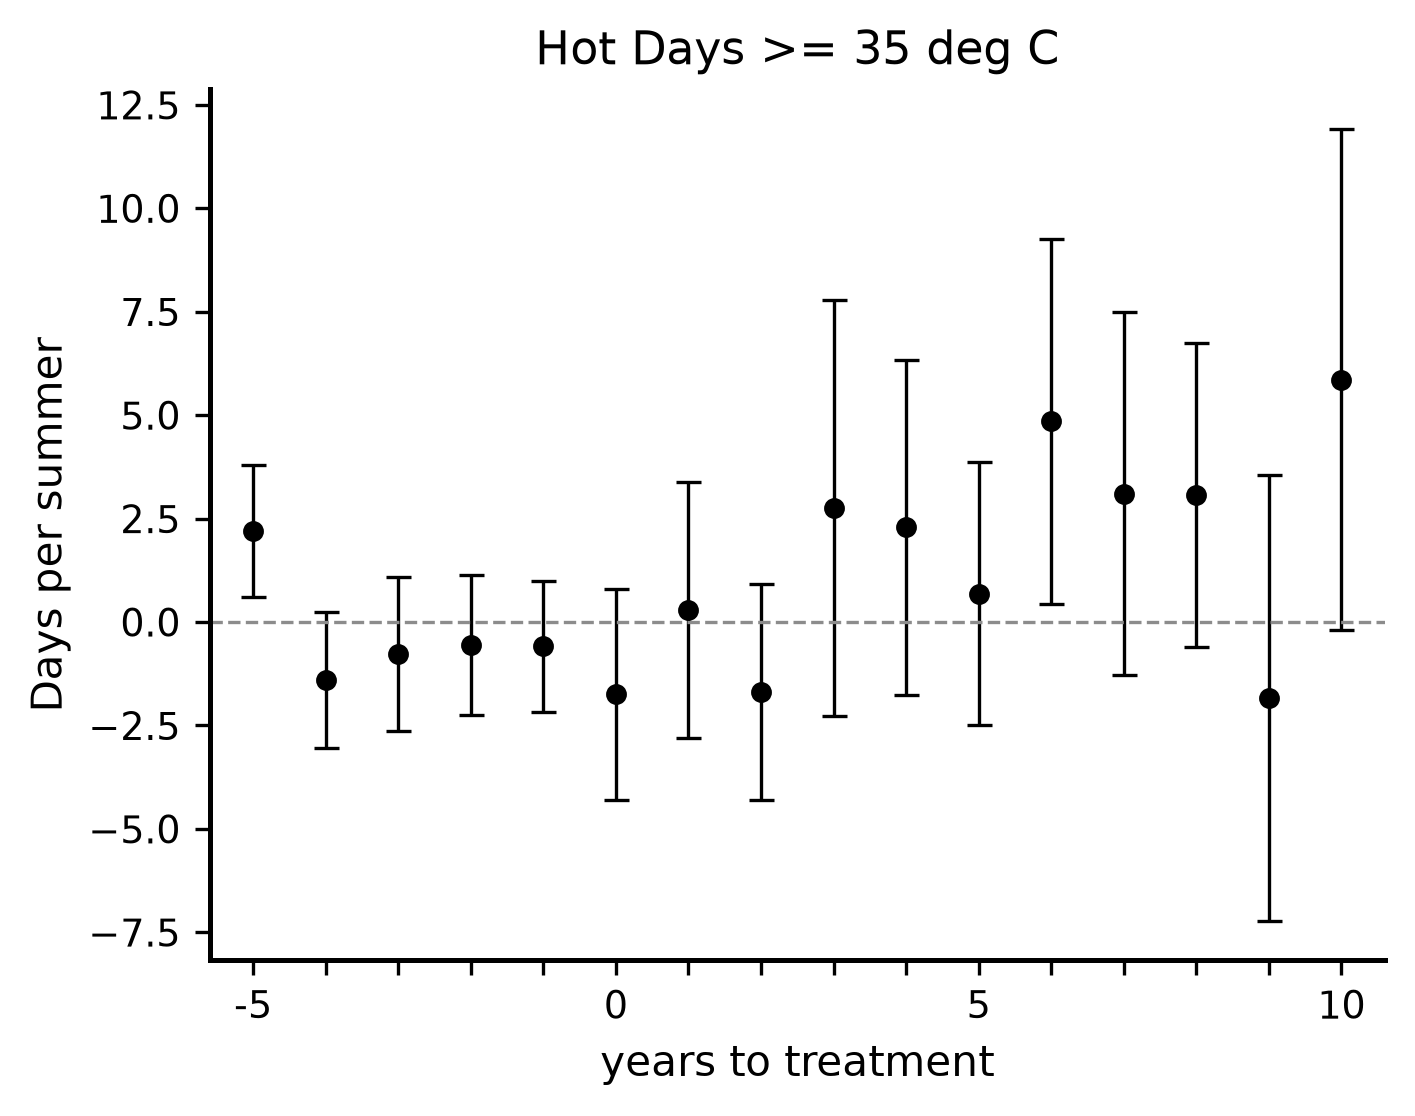
\includegraphics[width=0.47\textwidth]{station_event_study_bjs_dr_hot-days}
\end{tabular}
\end{singlespace}
\caption{Station-level BJS imputation with covariate adjustment (BJS with
controls) event studies, corresponding to column~(6) of
Table~\ref{tab:att}.  The horizontal axis shows years to treatment ($t = 0$
is the designation year, $t = -1$ is the reference period).  Dots are point
estimates; vertical whiskers show the 95\% confidence interval via sandwich
estimator.
\textit{Station Tmax ($^\circ$C)}: top left (summer mean daily maximum
temperature, GHCN-Daily \citep{Menne2012}).
\textit{NDVI (index)}: top right (MODIS NDVI at nearest pixel to each
station, MOD13A3 \citep{Didan2021}).
\textit{Tree cover (\%)}: bottom left (MODIS tree cover at nearest pixel,
MOD44B \citep{DiMiceli2021}).
\textit{Hot days (count)}: bottom right (annual days with Tmax
$\geq 35^\circ$C, GHCN-Daily).}
\label{fig:station_bjs}
\end{figure}

\end{document}
